%% LyX 1.6.9 created this file.  For more info, see http://www.lyx.org/.
%% Do not edit unless you really know what you are doing.
\documentclass[oneside,english]{amsart}
%\documentclass[oneside,english]{article}
\usepackage[T1]{fontenc}
\usepackage[utf8]{inputenc}
\usepackage{amsmath,amssymb,graphicx}
\usepackage{amsthm}
\usepackage{graphicx}
\usepackage{siunitx}
\usepackage{tikz}
%\usepackage{subfigure}
%\usepackage{epsfig}
%\usepackage{color}
%%%%%%%%%%%%%%%%%%%%%%%%%%%%%%%%%%%%%%%%%%%%%%%%
\graphicspath{{./Images/}}
%usepackage[dvips]{color}
%%%%%%%%%%%%%%%%%%%%%%%%%%%%%%%%%%%%%%%%%%%%%%%%%%%%%
\usepackage[left=2.5cm,right=2.5cm,top=3cm,bottom=3cm]{geometry}
%%%%%%%%%%%%%%%%%%%%%%%%%%%%%%%%%%%%%%%%%%%%%%%%%%%
%\newcommand{\cal}{\mathcal}
\newcommand{\beq}{\begin{equation}}
\newcommand{\eeq}{\end{equation}}
%%%%%%%%%%%%%%%%%%%%%%%%%%%%%%%%%%%%%%%%%%%%%%%%%%%%%
\def\sinc{\mathop{\rm sinc}\nolimits}  
\def\cal{\mathop{\rm cal}\nolimits}  
\def\cal{\mathop{\rm cal}\nolimits}  
\def\CFL{\mathop{\rm CFL}\nolimits}  
\def\ex{\mathop{\rm ex}\nolimits}  
\def\atan{\mathop{\rm atan}\nolimits}  
\def\sech{\mathop{\rm sech}\nolimits}  
\def\tanh{\mathop{\rm tanh}\nolimits}  
\def\div{\mathop{\rm div}\nolimits}  
\def\days{\mathop{\rm days}\nolimits}  
\def\Re{\mathop{\rm Re}\nolimits}  
\def\Sp{\mathop{\rm Sp}\nolimits}  
\newcommand{\bgrad}{\mbox{\boldmath$\nabla$}}
\newcommand{\bnabla}{\mbox{\boldmath$\nabla$}}
\newcommand{\bF}{\mbox{\boldmath$F$}}
\newcommand{\bP}{\mbox{\boldmath$P$}}
\newcommand{\bJ}{\mbox{\boldmath$J$}}
\newcommand{\bM}{\mbox{\boldmath$M$}}
\newcommand{\bg}{\mbox{\boldmath$g$}}
\newcommand{\bq}{\mbox{\boldmath$q$}}
\newcommand{\bx}{\mbox{\boldmath$x$}}
\newcommand{\bc}{\mbox{\boldmath$c$}}
\newcommand{\be}{\mbox{\boldmath$e$}}
\newcommand{\bn}{\mbox{\boldmath$n$}}
\newcommand{\bu}{\mbox{\boldmath$u$}}
\newcommand{\bv}{\mbox{\boldmath$v$}}
\newcommand{\bs}{\mbox{\boldmath$s$}}
\newcommand{\bi}{\mbox{\boldmath$i$}}
\newcommand{\bj}{\mbox{\boldmath$j$}}
%\newcommand{\bJ}{\mbox{\boldmath$J$}}
\newcommand{\bk}{\mbox{\boldmath$k$}}
\newcommand{\bvarphi}{\mbox{\boldmath$\varphi$}}
\newcommand{\bomega}{\mbox{\boldmath$\omega$}}
\newcommand{\bpsi}{\mbox{\boldmath$\psi$}}
%%%%%%%%%%%%%%%%%%%%%%%%%%%%%%%%%%%%%%%%%%%
    \newcommand{\cJ}{\mbox{\mathcal{J}}}
    \newcommand{\fu}{\mathfrak{u}}
    \newcommand{\fv}{\mathfrak{v}}
    \newcommand{\fw}{\mathfrak{w}}
    \newcommand{\fz}{\mathfrak{z}}
    \newcommand{\fe}{\mathfrak{e}}
    \newcommand{\fr}{\mathfrak{r}}
    \newcommand{\fg}{\mathfrak{g}}
    \newcommand{\fq}{\mathfrak{q}}
%%%%%%%%%%%%%%%%%%%%%%%%%%%%%%%%%%%%%%%%%%%%%
% ** PERSONAL NEWTHEOREMS
\newtheorem{thm}{Theorem}[section]
\theoremstyle{definition}
\newtheorem{defi}[thm]{Definition}
\newtheorem{prop}[thm]{Proposition}
\theoremstyle{remark}
\newtheorem{remark}[thm]{Remark}

\def\gint{\displaystyle\int}

\usepackage[ruled]{algorithm}
\usepackage{algpseudocode}
\alglanguage{pseudocode}


\makeatother

\usepackage{babel}

\begin{document}

\title{Numerical simulation of propagation problems on the sphere using a compact scheme}

\begin{abstract}
In this paper we continue the study of the compact scheme 
on the sphere introduced in 
\cite{Croisille-10, Croisille-12}. This scheme uses 
discrete differential operators on the Cubed Sphere. 
Considering propagation problems, the scheme is fully centered
and used a symmetric filter to eliminate high frequency
oscillating modes.
Numerical results on a broad series of numerical test cases
in climatology are presented, including
linear convection problems, the linearized shallow water 
and the non linear shallow water equations. 
These results demonstrate the
potential of the present approach 
in a variety of situations of interest accuracy and the 
stability of the present approach.
\end{abstract}

\author{M. Brachet and J.-P. Croisille\dag\ddag}
\address{\dag Universit\'e de Lorraine, D\'epartement de Math\'ematiques, F-57045 Metz, France\\
\ddag C.N.R.S., Institut Elie Cartan de Lorraine, UMR 7502, F-57045 Metz, France}
\email{matthieu.brachet@univ-lorraine.fr, jean-pierre.croisille@univ-lorraine.fr}
\date{November 2-nd, 2017}
\maketitle

{\sl Keywords: Cubed-Sphere grid - Compact finite difference scheme - 
Hermitian derivative - Vortex propagation}

%% **********************************************************************************************************************************************
\section{Introduction}
\label{sec:1}
In this paper, we continue the development
of the compact scheme introduced in \cite{Croisille-10,Croisille-12}
for the numerical resolution of 
partial differential equations on the sphere.
We are interested in propagation equations in 
climatology (atmosphere and ocean), 
which are related in a way or another
to the spherical Shallow Water equations (SWE).
These equations represent the reference hyperbolic system
to be solved in spherical geometry. 
A second problem (LSWE) is the linearized (SWE) 
around an atmosphere at rest. On this problem and its importance
in climatology and oceanography,
we refer to the recent monograph \cite{Paldor} and the references
therein.

Equations SWE or LSWE on the sphere are the source of many efforts
to adapt conservative methods  
originating from numerical gas dynamics.
This is in particular the case of the finite volume
method \cite{Chen-Xiao, Ullrich-Jablonowski-vanLeer}.
or the Discontinuous Galerkin methods \cite{Bao-Nair-Tufo}.
Conservative methods 
are designed to be applied to the conservative form 
of the equations.
However quantities,
which are theoretically conserved by SWE,
such as  energy, potential enstrophy angular momentum
can suffer excessive dissipation.
The effective numerical conservation of 
these quantities for large time largely depends of the
built-in dissipation of the scheme. 

The numerical scheme we are considering here is a 
finite difference scheme
scheme over the Cubed Sphere grid. 
Among the methods 
for fluid flows, this approach is related to 
the approximation of aeroacoustic equations by compact schemes,
along the lines of \cite{Lele, Visbal-Gaitonde, 
Tam-Webb, Bogey-Bailly}. This kind of approximation is also used
in the direct simulation of turbulence 
in parallelepipedic geometries \cite{Kim-Moin}.
Therefore our approach belongs to
a classical approach of computational fluid dynamics
which can be traced back to early works
in approximation and interpolation theory, \cite{Collatz}.
In the particular field of numerical climatology, 
it is related to \cite{Arakawa} and more recently
to the compact scheme presented in \cite{Ghader-Nordstrom}.

The convective problems considered here 
are of three types.
\begin{itemize}
\item 
The linear scalar advection equation 
\begin{equation}
\label{eq:adv}
\dfrac{\partial h}{\partial t}  (t,\mathbf{x})+ \mathbf{c}(t,\mathbf{x}) 
\cdot \nabla_T h(t,\mathbf{x})=0
\end{equation}
In (\ref{eq:adv}), the velocity 
$\mathbf{c} : (t,\mathbf{x}) \in (0, +\infty) \times \mathbb{S}^2 \mapsto \mathbf{c}(t,\mathbf{x}) \in \mathbb{T}\mathbb{S}^2$ 
is prescribed so that the scalar value $h(t,\mathbf{x})$ 
exhibits two moving antipodal vortices \cite{Nair-Machenhauer,Nair-Jablonowski}.
This problem goes beyond the classical solid body rotation test case.
The analytical solution permits a sharp
evaluation and comparison of any numerical scheme
for (\ref{eq:adv}).
\item
The LSWE system around the atmosphere at rest $q_0=[H_0,\mathbf{v}_0=\mathbf{0}]$
with $H_0 >0$ a constant height, 
is expressed as:
\begin{equation}
\label{eq:lswe}
(LSWE) \left\{
\begin{array}{l}
\dfrac{\partial \eta}{\partial t} (t,\mathbf{x})+ H \nabla_T 
\cdot \mathbf{v}(t,\mathbf{x})=0\\
\dfrac{\partial \mathbf{v} }{\partial t} (t,\mathbf{x})+ 
g \nabla_T \eta(t,\mathbf{x}) + f(\mathbf{x}) \mathbf{k}(\mathbf{x}) \times
\mathbf{v}(t,\mathbf{x})=0\\
\end{array}
\right.
\end{equation}
The state at rest is 
$(h_0,\mathbf{v}_0)=(H,\mathbf{0})$ and 
the 3-components unknowns is
the perturbation 
$(t,\mathbf{x}) \mapsto ( \eta(t,\mathbf{x}), \mathbf{v}(t,\mathbf{x}))$.
\item The SWE system is nonlinear. Its vector form is:
\begin{equation}
\label{eq:swe}
(SWE) \left\lbrace
\begin{array}{l}
\dfrac{\partial h^{\star}}{\partial t} (t,\mathbf{x}) + \nabla_T \cdot \left( h^{\star}(t,\mathbf{x}) \mathbf{v}(t,\mathbf{x}) \right) =  0 \\
\dfrac{\partial \mathbf{v}}{\partial t}  (t,\mathbf{x}) + \nabla_T \left( \dfrac{1}{2} |\mathbf{v}(t,\mathbf{x})|^2 
+ g h(t,\mathbf{x}) \right) + \left( f(\mathbf{x}) + \zeta(t,\mathbf{x}) \right) \mathbf{n}(\mathbf{x}) \times \mathbf{v}(t,\mathbf{x}) =  \mathbf{0} 
\end{array}
\right.
\end{equation}
where $\zeta = \left( \nabla_T \times \mathbf{v} \right) \cdot \mathbf{n}$ 
is the {\it relative vorticity} and 
$h^{\star} = h - h_s$ with $h_s$ the bottom topography function.
\end{itemize}

The form (\ref{eq:swe}) is nonconservative. 
It is adopted here, mainly
due to the fact that the gradient term 
is attractive to handle numerically
compared to the conservative form, \cite{Bao-Nair-Tufo}.
Equations (\ref{eq:adv}), (\ref{eq:lswe}) and (\ref{eq:swe}) 
are used in many benchmark test cases in numerical climatology.

For these three convective models, 
we show that our centered scheme is numerically competitive 
compared to conservative upwind methods.
Since the scheme is not a priori conservative,
we show careful evaluation in time of the conserved quantities.

The outline of the paper is as follows.
In Section \ref{sec:2}, we recall the essential of 
our approach introduced in 
\cite{Croisille-10, Croisille-12}. In \ref{sec:num}, we present 
numerical results on a series of test cases
relevant for the three systems of equations above. After concluding in \ref{sec:conclu}, we add numerical analysis of the advected problem is 1D periodic in \ref{sec:annexes}. 


















%% **********************************************************************************************************************************************
\section{Numerical scheme using central compact differencing 
on the Cubed Sphere}
\label{sec:2}
In this section, after a brief overview of 
the Cubed Sphere in Section
\ref{sec:CS}, the essential of
our central differencing approach using a compact scheme
is summarized in Section \ref{sec:der_cs}.
In Section \ref{sec:op} a discrete counterpart 
of the operators gradient, divergence and curl
are deduced from this central differencing
is derived.

%% **********************************************************************************************************************************************
\subsection{The Cubed-Sphere}
\label{sec:CS}
The Cubed Sphere is a spherical grid widely used
in numerical climatology since \cite{Sadourny}.
A modern 
presentation was given in
\cite{Ronchi-Iacono-Paolucci}.
It is composed of six panels (six charts) 
labeled $(k)=(I), (II), (II), (IV), (V)$ and $(VI)$. Each panel 
matches
the face of a cube and
supports a Cartesian grid of size $(N+1)\times (N+1)$.
It is equipped with a 
coordinate system $(\xi,\eta)$
whose coordinate lines are two "equatorial" angles identified along a couple of orthogonal great circles
intersecting at the center of the panel. 
The Cubed Sphere is represented on Fig. \ref{fig:1}
and a typical panel is shown
on Fig. \ref{fig:2}.
The resolution parameter is denoted by $N$,
which denotes the number of cells in each direction $\xi$ or $\eta$ on each panels. 
The points are denoted 
$\mathbf{s}_{i,j}^{(k)}$
The integer $i$ (resp. $j$) 
denotes the index in the $\xi$ direction (resp. $\eta$) direction and 
$(k)\in (I)...(VI)$ denotes the panel. Our finite difference scheme 
hereafter uses discrete unknowns
located at the points $\mathbf{s}^{(k)}_{i,j}$ and therefore it uses $6 N^2+2$ unknowns,
i.e. the number of points on the Cubed Sphere.

%% **********************************************************************************************************************************************
\subsection{Great circles on the Cubed Sphere}
\label{sec:der_cs}
The  main idea of our approximation consists
of using great circles on the Cubed Sphere. Each circle is associated to a panel. 
Two typical great circles are represented
on figure \ref{fig:patron cs} in blue and red.

\begin{figure}
\begin{center}
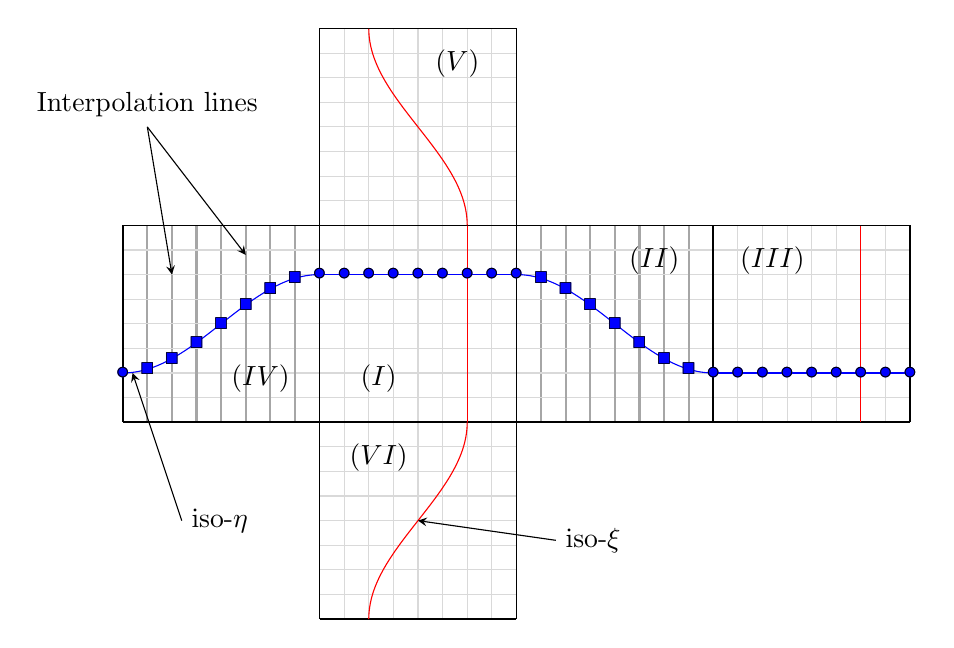
\begin{tikzpicture}[scale=2.5]
	\foreach \x in {1,...,7}
		{ \draw [color=gray!70, line width=0.8pt] (0.125*\x,1) -- (0.125*\x,2) ;
		\draw [color=gray!30] (0,1+0.125*\x) -- (1,1+0.125*\x) ;
		\draw [color=gray!30] (1+0.125*\x,1) -- (1+0.125*\x,2) ;
		\draw [color=gray!30] (1,1+0.125*\x) -- (2,1+0.125*\x) ;
		\draw [color=gray!70, line width=0.8pt] (2+0.125*\x,1) -- (2+0.125*\x,2) ;
		\draw [color=gray!30] (2,1+0.125*\x) -- (3,1+0.125*\x) ;
		\draw [color=gray!30] (3+0.125*\x,1) -- (3+0.125*\x,2) ;
		\draw [color=gray!30] (3,1+0.125*\x) -- (4,1+0.125*\x) ;
		\draw [color=gray!30] (1+0.125*\x,0) -- (1+0.125*\x,1) ;
		\draw [color=gray!30] (1,0.125*\x) -- (2,0.125*\x) ;
		\draw [color=gray!30] (1+0.125*\x,2) -- (1+0.125*\x,3) ;		
		\draw [color=gray!30] (1,2+0.125*\x) -- (2,2+0.125*\x) ;
		}
	

	\draw [line width=0.6pt] (1,3) -- (2,3) ; 
	\draw [line width=0.6pt] (0,2) -- (4,2) ; 	
	\draw [line width=0.6pt] (0,1) -- (4,1) ; 
	\draw [line width=0.6pt] (1,0) -- (2,0) ; 
	
	\draw [line width=0.6pt] (0,2) -- (0,1) ;
	\draw [line width=0.6pt] (1,3) -- (1,0) ;
	\draw [line width=0.6pt] (2,3) -- (2,0) ;
	\draw [line width=0.6pt] (3,2) -- (3,1) ;
	\draw [line width=0.6pt] (4,2) -- (4,1) ; 
	
	\draw (0.7,1.1) node[above]{$(IV)$} ; 
	\draw (1.3,1.1) node[above]{$(I)$} ; 
	\draw (2.7,1.7) node[above]{$(II)$} ;
	\draw (3.3,1.7) node[above]{$(III)$} ;  
	\draw (1.7,2.7) node[above]{$(V)$} ;  
	\draw (1.3,0.7) node[above]{$(VI)$} ; 
	
	\draw [samples=100,domain=0:1,color=blue] plot({\x},{1.5-(2*0.125)*cos(180*\x)});
	\draw [samples=100,domain=1:2,color=blue] plot({\x},{1.5+2*0.125});
	\draw [samples=100,domain=1:2,color=blue] plot({\x+1},{1.5-2*0.125*cos(180*\x)});
	\draw [samples=100,domain=3:4,color=blue] plot({\x},{1.5-2*0.125});
	\draw [>=stealth, <-] (0.05,1.25) -- (0.3,0.5) ;
	\draw  (0.3,0.5) node[right] {iso-$\eta$} ;
	
	\draw [samples=100,domain=0:1,color=red] plot({1.5-2*0.125*cos(180*\x)},{\x});
	\draw [samples=100,domain=1:2,color=red] plot({1.5+2*0.125},{\x});
	\draw [samples=100,domain=1:2,color=red] plot({1.5-2*0.125*cos(180*\x)},{\x+1});
	\draw [samples=100,domain=1:2,color=red] plot({4-+2*0.125},{\x});
	\draw [>=stealth, <-] (1.5,0.5) -- (2.2,0.4) ;
	\draw  (2.2,0.4) node[right] {iso-$\xi$} ;
	
	\draw  (0,1+2*0.125) node[color=blue] {$\bullet$} ;
	\draw (0,1+2*0.125) node {$\circ$} ;
	
	\foreach \k in {0,...,8}
		{\draw  (1+0.125*\k,1.5+2*0.125) node[color=blue] {$\bullet$} ;
	   	\draw (1+0.125*\k,1.5+2*0.125) node {$\circ$} ;
	   	\draw  (3+0.125*\k,1+2*0.125) node[color=blue] {$\bullet$} ;
	   	\draw (3+0.125*\k,1+2*0.125) node {$\circ$} ;
	   	}
	   	
	\foreach \x in {1,...,7}
		{\draw  ({0.125*\x},{1.5-2*0.125*cos(180*0.125*\x)}) node[color=blue] {\begin{tiny}$\blacksquare$\end{tiny}} ;
	   	\draw ({0.125*\x},{1.5-2*0.125*cos(180*0.125*\x)}) node {\begin{tiny}$\square$\end{tiny}} ;
	   	\draw  ({2+0.125*\x},{1.5-2*0.125*cos(180*0.125*\x+180)}) node[color=blue] {\begin{tiny}$\blacksquare$\end{tiny}} ;
	   	\draw  ({2+0.125*\x},{1.5-2*0.125*cos(180*0.125*\x+180)}) node {\begin{tiny}$\square$\end{tiny}} ;
	   	}
	   	
	\draw [>=stealth, <-] (0.25,1.75) -- (0.125,2.5) ;
	\draw [>=stealth, <-] (0.625,1.85) -- (0.125,2.5) ;
	\draw  (0.125,2.5) node[above] {Interpolation lines} ;
\end{tikzpicture}
\caption{Greats circles associated to the panel $(I)$ and $(III)$ are completed with data from interpolation lines on panels $(II)$ and $(IV)$.}
\label{fig:patron cs}
\end{center}
\end{figure}




\begin{figure}[htbp]
\begin{center}
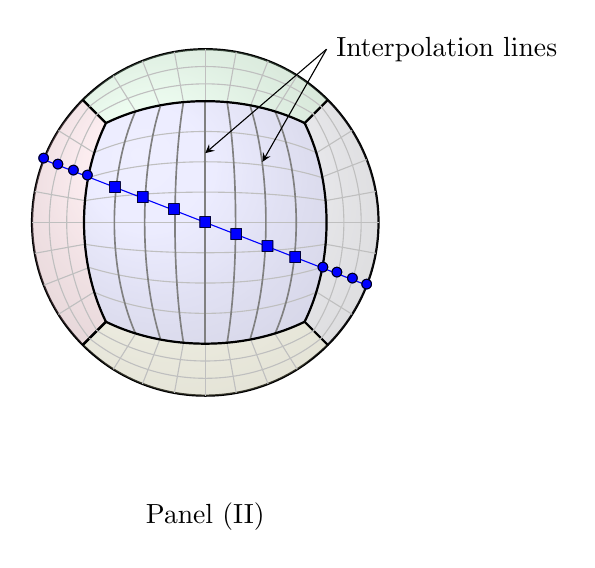
\begin{tikzpicture}[scale=2.2]
	\draw [line width=0.8pt] (0,0) circle (1cm);
    \shade[ball color=blue!10!white,opacity=0.20] (0,0) circle (1cm);	
	
	\filldraw[draw=black,fill=blue!30!white,opacity=0.20]
	plot [smooth,domain=-35:35] ({0.7*cos(\x)},{sin(\x)})
	-- plot [smooth,domain=55:125] ({cos(\x)},{0.7*sin(\x)})
	-- plot [smooth,domain=150:215] ({0.7*cos(\x)},{sin(\x)})
	-- plot [smooth,domain=240:300] ({cos(\x)},{0.7*sin(\x)})
	-- cycle;	
	\draw [samples=100,domain=48:132, color=gray!50] plot({cos(\x)},{0.35*sin(\x)});
	\draw [samples=100,domain=48:132, color=gray!50] plot({cos(\x)},{-.35*sin(\x)});
	\draw [samples=100,domain=46:134, color=gray!50] plot({cos(\x)},{0.175*sin(\x)});
	\draw [samples=100,domain=46:134, color=gray!50] plot({cos(\x)},{-.175*sin(\x)});
	\draw [samples=100,domain=50:130, color=gray!50] plot({cos(\x)},{0.525*sin(\x)});
	\draw [samples=100,domain=50:130, color=gray!50] plot({cos(\x)},{-.525*sin(\x)});
	\draw [samples=100,domain=45:135, color=gray!50] plot({cos(\x)},{0*sin(\x)});

	\draw [rotate=90, samples=100,domain=48:132, color=gray, line width=0.6pt] plot({cos(\x)},{0.35*sin(\x)});
	\draw [rotate=90, samples=100,domain=48:132, color=gray, line width=0.6pt] plot({cos(\x)},{-.35*sin(\x)});
	\draw [rotate=90, samples=100,domain=46:134, color=gray, line width=0.6pt] plot({cos(\x)},{0.175*sin(\x)});
	\draw [rotate=90, samples=100,domain=46:134, color=gray, line width=0.6pt] plot({cos(\x)},{-.175*sin(\x)});
	\draw [rotate=90, samples=100,domain=50:130, color=gray, line width=0.6pt] plot({cos(\x)},{0.525*sin(\x)});
	\draw [rotate=90, samples=100,domain=50:130, color=gray, line width=0.6pt] plot({cos(\x)},{-.525*sin(\x)});
	\draw [rotate=90, samples=100,domain=45:135, color=gray, line width=0.6pt] plot({cos(\x)},{0*sin(\x)});

	\filldraw[draw=black,fill=red!30!white,opacity=0.20]
	plot [smooth,domain=145:215] ({.7*cos(\x)},{sin(\x)})
	-- plot [smooth] (-.573,-.573) -- (-.707,-.707)
	-- plot [smooth,domain=215:145] ({cos(\x)},{sin(\x)})
	-- plot [smooth] (-.707,.707) -- (-.573,.573)
	-- cycle;	
	\draw [line width=0.8pt] (-.573,-.573) -- (-.707,-.707) ;
	\draw [line width=0.8pt] (-.573,.573) -- (-.707,.707) ;
	\draw [color=gray!50] (-.669,.260) -- (-.9321,.3622) ;
	\draw [color=gray!50] (-.669,-.260) -- (-.9321,-.3622) ;
	\draw [color=gray!50] (-.6946,.1259) -- (-.9840,.1783) ;
	\draw [color=gray!50] (-.6946,-.1259) -- (-.9840,-.1783) ;
	\draw [color=gray!50] (-.6427,.4022) -- (-.8477,.5305) ;
	\draw [color=gray!50] (-.6427,-.4022) -- (-.8477,-.5305) ;
	\draw [color=gray!50] (-.707,0) -- (-1,0) ;
	\draw [samples=100,domain=141:219, color=gray!50] plot({0.8*cos(\x)},{sin(\x)});
	\draw [samples=100,domain=138:222, color=gray!50] plot({0.9*cos(\x)},{sin(\x)});
	
	\filldraw[draw=black,fill=green!30!white,opacity=0.20]
	plot [smooth,domain=55:125] ({cos(\x)},{0.7*sin(\x)})
	-- plot [smooth] (-.573,.573) -- (-.707,.707)
	-- plot [smooth,domain=125:55] ({cos(\x)},{sin(\x)})
	-- plot [smooth] (.707,.707) -- (.573,.573)
	-- cycle;	
	\draw [line width=0.8pt] (-.573,.573) -- (-.707,.707) ;
	\draw [line width=0.8pt] (.707,.707) -- (.573,.573) ;
	\draw [rotate=-90,color=gray!50] (-.669,.260) -- (-.9321,.3622) ;
	\draw [rotate=-90,color=gray!50] (-.669,-.260) -- (-.9321,-.3622) ;
	\draw [rotate=-90,color=gray!50] (-.6946,.1259) -- (-.9840,.1783) ;
	\draw [rotate=-90,color=gray!50] (-.6946,-.1259) -- (-.9840,-.1783) ;
	\draw [rotate=-90,color=gray!50] (-.6427,.4022) -- (-.8477,.5305) ;
	\draw [rotate=-90,color=gray!50] (-.6427,-.4022) -- (-.8477,-.5305) ;
	\draw [rotate=-90,color=gray!50] (-.707,0) -- (-1,0) ;
	\draw [rotate=-90,samples=100,domain=141:219, color=gray!50] plot({0.8*cos(\x)},{sin(\x)});
	\draw [rotate=-90,samples=100,domain=138:222, color=gray!50] plot({0.9*cos(\x)},{sin(\x)});
	
	\filldraw[draw=black,fill=yellow!30!white,opacity=0.20]
	plot [smooth,domain=55:125] ({cos(\x)},{-.7*sin(\x)})
	-- plot [smooth] (-.573,-.573) -- (-.707,-.707)
	-- plot [smooth,domain=125:55] ({cos(\x)},{-sin(\x)})
	-- plot [smooth] (.707,-.707) -- (.573,-.573)
	-- cycle;	
	\draw [line width=0.8pt] (-.573,-.573) -- (-.707,-.707) ;
	\draw [line width=0.8pt] (.707,-.707) -- (.573,-.573) ;
	\draw [rotate=90,color=gray!50] (-.669,.260) -- (-.9321,.3622) ;
	\draw [rotate=90,color=gray!50] (-.669,-.260) -- (-.9321,-.3622) ;
	\draw [rotate=90,color=gray!50] (-.6946,.1259) -- (-.9840,.1783) ;
	\draw [rotate=90,color=gray!50] (-.6946,-.1259) -- (-.9840,-.1783) ;
	\draw [rotate=90,color=gray!50] (-.6427,.4022) -- (-.8477,.5305) ;
	\draw [rotate=90,color=gray!50] (-.6427,-.4022) -- (-.8477,-.5305) ;
	\draw [rotate=90,color=gray!50] (-.707,0) -- (-1,0) ;
	\draw [rotate=90,samples=100,domain=141:219, color=gray!50] plot({0.8*cos(\x)},{sin(\x)});
	\draw [rotate=90,samples=100,domain=138:222, color=gray!50] plot({0.9*cos(\x)},{sin(\x)});
	
	\draw [rotate=180,color=gray!50] (-.669,.260) -- (-.9321,.3622) ;
	\draw [rotate=180,color=gray!50] (-.669,-.260) -- (-.9321,-.3622) ;
	\draw [rotate=180,color=gray!50] (-.6946,.1259) -- (-.9840,.1783) ;
	\draw [rotate=180,color=gray!50] (-.6946,-.1259) -- (-.9840,-.1783) ;
	\draw [rotate=180,color=gray!50] (-.6427,.4022) -- (-.8477,.5305) ;
	\draw [rotate=180,color=gray!50] (-.6427,-.4022) -- (-.8477,-.5305) ;
	\draw [rotate=180,color=gray!50] (-.707,0) -- (-1,0) ;
	\draw [rotate=180,samples=100,domain=141:219, color=gray!50] plot({0.8*cos(\x)},{sin(\x)});
	\draw [rotate=180,samples=100,domain=138:222, color=gray!50] plot({0.9*cos(\x)},{sin(\x)});
	
	\draw [samples=100,domain=55:125, line width=0.8pt] plot({cos(\x)},{0.7*sin(\x)});
	\draw [samples=100,domain=55:125, line width=0.8pt] plot({cos(\x)},{-.7*sin(\x)});
	\draw [samples=100,domain=145:215, line width=0.8pt] plot({.7*cos(\x)},{sin(\x)}); 
	\draw [samples=100,domain=145:215, line width=0.8pt] plot({-.7*cos(\x)},{sin(\x)}); 
	
	\draw [color=blue] (-.9321,.3622) -- (.9321,-.3622) ;
	\draw  (-.9321,.3622) node[color=blue] {$\bullet$} ;
	\draw (-.9321,.3622) node {$\circ$} ;	
	\draw  (.9321,-.3622) node[color=blue] {$\bullet$} ;
	\draw (.9321,-.3622) node {$\circ$} ;
	\draw  (-.85,0.3886*.85) node[color=blue] {$\bullet$} ;
	\draw (-.85,0.3886*.85) node {$\circ$} ;	
	\draw (.85,-0.3886*.85) node[color=blue] {$\bullet$} ;
	\draw (.85,-0.3886*.85) node {$\circ$} ;	
	\draw  (-.76,0.3886*.76) node[color=blue] {$\bullet$} ;
	\draw (-.76,0.3886*.76) node {$\circ$} ;	
	\draw (.76,-0.3886*.76) node[color=blue] {$\bullet$} ;
	\draw (.76,-0.3886*.76) node {$\circ$} ;
	\draw  (-.68,0.3886*.68) node[color=blue] {$\bullet$} ;
	\draw (-.68,0.3886*.68) node {$\circ$} ;	
	\draw (.68,-0.3886*.68) node[color=blue] {$\bullet$} ;
	\draw (.68,-0.3886*.68) node {$\circ$} ;	
	\draw (-.52,0.3886*.52) node[color=blue] {\begin{tiny}$\blacksquare$ \end{tiny}} ;
	\draw (-.52,0.3886*.52) node {\begin{tiny}$\square$ \end{tiny}} ;
	\draw (.52,-0.3886*.52) node[color=blue] {\begin{tiny}$\blacksquare$ \end{tiny}} ;
	\draw (.52,-0.3886*.52) node {\begin{tiny}$\square$ \end{tiny}} ;
	\draw (-.36,0.3886*.36) node[color=blue] {\begin{tiny}$\blacksquare$ \end{tiny}} ;
	\draw (-.36,0.3886*.36) node {\begin{tiny}$\square$ \end{tiny}} ;
	\draw (.36,-0.3886*.36) node[color=blue] {\begin{tiny}$\blacksquare$ \end{tiny}} ;
	\draw (.36,-0.3886*.36) node {\begin{tiny}$\square$ \end{tiny}} ;
	\draw (-.18,0.3886*.18) node[color=blue] {\begin{tiny}$\blacksquare$ \end{tiny}} ;
	\draw (-.18,0.3886*.18) node {\begin{tiny}$\square$ \end{tiny}} ;
	\draw (.18,-0.3886*.18) node[color=blue] {\begin{tiny}$\blacksquare$ \end{tiny}} ;
	\draw (.18,-0.3886*.18) node {\begin{tiny}$\square$ \end{tiny}} ;
	\draw (0,0) node[color=blue] {\begin{tiny}$\blacksquare$ \end{tiny}} ;
	\draw (0,0) node {\begin{tiny}$\square$ \end{tiny}} ;
	
	\draw [>=stealth, <-] (.33,.35) -- (.7,1) ;
	\draw [>=stealth, <-] (0,.4) -- (.7,1) ;
	\draw  (0.7,1) node[right] {Interpolation lines} ;
	
	\draw  (0,-1.7) node {Panel (II)} ;

\end{tikzpicture}
\end{center}
\caption{The blue line is a great circle associated with panel $(I)$ and view by the panel $(II)$. Blue circle represent points on the Cubed-sphere, blue squares do not belong the Cubed-Sphere.}
\label{fig: panel II_interp}
\end{figure}  


This circles coincide with coordinate lines on panels $(I)$ and $(III)$. In the contrary, they do not coincide with coordinate lines on panels (II) and (IV).
On panel $(k)$, $(I) \leq (k) \leq (VI)$, the local basis is 
\beq
\label{eq:32.19}
\bg_\xi(\mathbf{x})=\frac{\partial \mathbf{x}}{\partial \xi},\;\;\;
\bg_\eta(\mathbf{x})=\frac{\partial \mathbf{x}}{\partial \eta}.
\eeq
and the dual basis is called $(\bg^\xi, \bg^\eta)$.
Consider a regular function $f : \mathbf{x} \in \mathbb{S}^2_a \mapsto f(x) \in \mathbb{R}$ on the sphere.
The gradient of $f$ is
\begin{equation}
\nabla_T f = \dfrac{\partial f}{\partial \xi} \mathbf{g}^{\xi} + \dfrac{\partial f}{\partial \eta} \mathbf{g}^{\eta}
\label{eq:gradient}
\end{equation}
Consider the restriction $f^k_{i,j} = f(\mathbf{s}_{i,j}^k)$ to the Cubed-sphere. The approximate gradient is
\begin{equation}
\nabla_{T,h} f_{i,j}^k =f_{\xi, i,j}^k \mathbf{g}^{\xi} + f_{\eta,i,j}^k \mathbf{g}^{\eta}
\label{eq:gradient_app}
\end{equation}
In \eqref{eq:gradient_app}, the partial derivative $\frac{\partial}{\partial \xi} f_{i,j}^{(k)}$ is approximated by $f_{\xi,i,j}^{(k)}$ along a great circle.
Condiser for example the approximation of the derivative $\partial_{\xi}f_{i,j}^k$. We use the blue circle on figure \ref{fig:patron cs} and \ref{fig: panel II_interp} to illustrate the algorithm. This circle correspond to the iso-$\eta$ line $\eta=\eta_0$.

\begin{enumerate}
\item Define on the blue circle the grid $p = 0, ..., 4N$ as follow :
\begin{enumerate}
\item $m_p = s^{(I)}_{p-N/2,j_0}$, $p=0, ..., N-1$. These $N$ points are represented by blue circles on figure \ref{fig:patron cs}. They belong to the Cubed-Sphere,
\item $m_p$, $p=N...2N-1$. These points are represented by blue squares on panel $(II)$ on figure \ref{fig:patron cs}. They do not belong the Cubed-Sphere.
\item $m_p = s^{(III)}_{p-N/2,j_0}$, $p=2N, ..., 3N-1$. These $N$ points are represented by blue circles on figure \ref{fig:patron cs}. They belong to the Cubed-Sphere,
\item $m_p$, $p=3N...4N-1$. These points are represented by blue squares on panel $(IV)$, on figure \ref{fig:patron cs}. They do not belong the Cubed-Sphere.
\end{enumerate}

\item Interpolate data from the Cubed-sphere to the blue great circle as follow :
\begin{enumerate}
\item On panels $(I)$ and $(III)$, data are simply transfered,
\item On panels $(II)$ and $(IV)$, dara are interpolated (see \cite{Croisille-10}).
\end{enumerate}
The interpolation procedure adoped uses cubic-splines as follow :
\begin{enumerate}
\item the blue circle cross the iso$-\xi$ lines on panel $(II)$ and $(IV)$ (interpolation lines), 
\item we use a cubic spline to complete the data on each cross point (represented by blue square on figure \ref{fig: panel II_interp}) using the data on the associated interpolation line.
\end{enumerate}

\item The hermitian discrete derivative $\delta_{\xi}^H$ is applied to the data assembled along great the blue circle (the hermitian scheme is detailled in \ref{sec:annexes}). This step provides $4N$ values called $v_{\xi, p}$, with $p=0, ..., 4N$. Periodicity ensures that $v_{\xi, 4N} = v_{\xi,0}$.

\item Finally retain the values $v_{\xi, p}$ with $0 \leq p \leq N$ and $2N \leq p \leq 3N$, which corresponds to panels $(I)$ and $(III)$.
\end{enumerate}

This procedure is applied to all iso-$\eta$ great circles $\eta_j = j \Delta \eta$ with $j = -N/2, ..., N/2$ of panel $(I)$. Then it is identically applied to all great circle of the following great circles :
\begin{itemize}
\item $(C_i^{(1)})_{- N/2 \leq i \leq N/2}$ are the iso-$\xi$ lines on each panel,
\item $(C_j^{(2)})_{- N/2 \leq j \leq N/2}$ are the iso-$\xi$ lines on each panel.
\end{itemize}
There are six sets of $N+1$ circles.

As a result, approximate values for $f_{\xi, i, j}$ and $f_{\eta, i, j}$ are obtained on the six panels. Using \ref{eq:gradient_app}, this allow to obtain an approximation of the gradient at each point of the Cubed-sphere.












\subsection{Approximation of spherical differential operators}
\label{sec:op}
Equations (\ref{eq:adv}), (\ref{eq:lswe}) and (\ref{eq:swe}) require
discrete tangential operators approximating
the gradient, the divergence and the curl. 
Our starting point is to perform 
three point compact differencing along a series of 
great circles on the Cubed Sphere.
This principle is particularly suited 
on the Cubed Sphere since on each panel,
coordinate lines are sections of great circles.
In addition, we take advantage of the periodic
setting along these great circles.
In particular, we avoid the definition of ghost points.
As already mentioned, the fundamental of our scheme
is to evaluate Hermitian derivatives
along a series of great circles on the sphere.
These great circles are associated to
coordinates lines on each panel.
In a second time, discrete differential operators are
deduced from them.
Details can be found in \cite{Croisille-10, Croisille-12}.


Let $\bx \in \mathbb{S}^2 \mapsto f(\bx)$ be a regular function.
The gradient is defined by
\beq
\nabla_T f= 
\partial_\xi f \bg^\xi +\partial_\eta f \bg^\eta
\eeq
Let $f^k_{i,j}$ 
be a given scalar gridfunction on the Cubed Sphere.
Denoting $h=\Delta \xi=\Delta \eta=\frac{\pi}{2N}$, we have
\beq
\label{eq:grad}
\nabla_{T,h} f= 
 f_{\xi,i,j}^k (\bg^\xi)_{i,j}^k 
+
f_{\eta,i,j}^k (\bg^\eta)_{i,j}^k 
\eeq

Similarly if 
$\bv: \bx \in \mathbb{S}^2 \mapsto \mathbb{T}\mathbb{S}^2$
is a regular tangential vector field,
the divergence and curl are:
\beq
\label{eq:95.13.1}
\left\{
\begin{array}{l}
\nabla_T \cdot \bv= 
\partial_\xi \bv \cdot  \bg^\xi +\partial_\eta \bv \cdot \bg^\eta\\
\nabla_T \times \bv = 
\partial_\xi \bv \times \bg ^\xi +\partial_\eta \bv \times \bg ^\eta
\end{array}
\right.
\eeq
The discrete divergence and curl of 
a discrete tangential vector grid function
$\bv^k_{i,j}$ are called 
$\nabla_{T,h} \cdot \bv_{i,j}^k$ 
and $\nabla_{T,h} \times\bv_{i,j}^k$ respectively.
They are defined by
\beq
\left\{
\begin{array}{l}
\nabla_{T,h} \cdot (\bv)_{i,j}^k= 
(\bv)_{\xi,i,j}^k \cdot  (\bg^\xi)_{i,j}^k 
+
\nabla_{T,h}
(\bv)^k_{i,j} \cdot (\bg^\eta)^k_{i,j}\\
\nabla_{T,h} \times (\bv)_{i,j}^k = 
(\bv)_{i,j}^k \times (\bg ^\xi)^k_{i,j} 
+
(\bv)_{i,j}^k \times (\bg ^\eta)^k_{i,j}
\end{array}
\right.
\label{eq:div_rot}
\eeq
Due to \eqref{eq:87.14.1}, we expect these discrete operators
to be fourth order accurate.

\begin{prop}
If $f(\bx)$ and $\bv(\bx)$ are any given scalar (resp. tangential vector)
function on the sphere. If $f^\ast$ and $\bv^\ast$
are their restriction to the Cubed Sphere, then the
consistency relations hold:
\beq
\label{eq:11.91}
\begin{aligned}
\nabla_{T,h} f^k_{i,j}-(\nabla_T f)^{\ast,k}_{i,j}&=\mathcal{O} (\Delta^3)\\
\nabla_{T,h} \cdot \bv^k_{i,j}
-(\nabla_T \cdot  f)^{\ast,k}_{i,j}&=\mathcal{O} (\Delta^3)\\
\nabla_{T,h} \times \bv^k_{i,j}
-(\nabla_T \times  \bv)^{\ast,k}_{i,j}&=\mathcal{O} (\Delta^3)
\end{aligned}
\eeq
\end{prop}
\begin{proof}
We prove the result for the gradient operator.
Let $f : \mathbf{x} \mapsto f(x) \in \mathbb{S}^2$ a regular function. Let $\mathbf{x}_p$ a point on an iso$-\eta$ and $f_p$ an approximation of $f(x_p)$.

Using the process to calculate the derivative $\partial_{\xi}f$ on the iso$-\xi$, there are two possibilities
\begin{enumerate}
\item $\mathbf{x}_p$ is on the cubed-sphere, then $f_p = f(x_p)$,
\item $\mathbf{x}_p$ is not on the grid. Because of the cubic-spline is ordre $4$, we have
\begin{equation}
f_p = f(x_p) + \mathcal{O}(\Delta \eta^4).
\end{equation}
\end{enumerate}
Then, on a given iso$-\eta$, the data are pertubated with the cubic spline and for all $0 \leq p \leq 4N-1$, 
\begin{equation}
f_p = f(x_p) + \mathcal{O}(\Delta \eta^4).
\end{equation}
Then,
\begin{equation}
\delta_{\xi} f_p = \dfrac{f_{p+1}-f_{p-1}}{2 \Delta \xi} =\dfrac{f(\mathbf{x}_{p+1})-f(\mathbf{x}_{p-1})}{2 \Delta \xi} + \mathcal{O}(\Delta \eta^3)
\end{equation}
and the result is
\begin{equation}
\delta_{\xi}^H f_p = \partial_{\xi} f(\mathbf{x}_p) + \mathcal{O}(\Delta \eta^3).
\end{equation}

In the same way, if $\mathbf{x}_k$ define a grid in an iso$-\xi$,
\begin{equation}
\delta_{\eta}^H f_k = \partial_{\eta} f(\mathbf{x}_k) + \mathcal{O}(\Delta \xi^3).
\end{equation}

Using this two previous formula and $\Delta \xi = \Delta \eta = \Delta$, the linearity of the gradient operator imply
\begin{equation}
\nabla_{T,h} f^k_{i,j}-(\nabla_T f)^{\ast,k}_{i,j}=\mathcal{O} (\Delta^3).
\end{equation}
The proof is similar for curl and divergence operator.
\end{proof}
\begin{figure}
\includegraphics[scale=0.4]{Images/fig6.jpg}
\caption{
The Cubed Sphere with grid parameter $N=16$.
The total number of gridpoints is $6 \times N^2+2=1538$ in this case.
The panels $(I)$, $(II)$, $(III)$ and $(IV)$ are located
around the equatorial plane $z=0$. The index of the north panel is $(V)$ 
and the one of the south panel is $(VI)$. 
}
\label{fig:1}
\end{figure}

\begin{figure}
   \def\svgwidth{0.3 \textwidth}
\input{drawing13.pdf_tex}
\caption{
The points of a typical panel of the Cubed-Sphere are classified in three categories:
(i) Circles correspond to {\sl internal} points; (ii) Squares correspond to {\sl edge} points ;
(iii) Pentagons correspond to {\sl corner} points}
\label{fig:2}
\end{figure}











%% **********************************************************************************************************************************************
\subsection{Method of lines}
Using the method of lines, the space discretization is made with the discrete operators \eqref{eq:grad} and \eqref{eq:div_rot}. 
Then, equations take the form 
\begin{equation}
\dfrac{d q}{dt} = J_{\Delta}(q)
\end{equation}
where $q = h$, restrict to the grid, for the advection equation \eqref{eq:adv}, $q=[\eta, \mathbf{v}]^T$ for the linearized shallow water equation \eqref{eq:lswe} and $q=[h, \mathbf{v}]^T$ for shallow water equation \eqref{eq:swe}.

For example, for the shallow water equation \eqref{eq:swe}, $q = [h_{i,j}^k, \mathbf{v}_{i,j}^k]^T$ with $-N/2 \leq i,j \leq N/2$ and $k = (I), ..., (VI)$. Each operator is approximated using (\ref{eq:grad} - \ref{eq:95.13.1}). Then
\begin{equation}
J_{\Delta}(q) = J_{\Delta}(h_{i,j}^k, \mathbf{v}_{i,j}^k) = 
\begin{bmatrix}
- \nabla_{T,h} \cdot \left( h^{\star k}_{i,j} \mathbf{v}_{i,j}^k \right) \\
- \nabla_{T,h} \left( \dfrac{1}{2} |\mathbf{v}_{i,j}^k|^2 
+ g h_{i,j}^k \right) - \left( f_{i,j}^k + \zeta_{i,j}^k \right) \mathbf{n}_{i,j}^k \times \mathbf{v}_{i,j}^k 
\end{bmatrix}
\end{equation}
with $\zeta_{i,j}^k = \left(\nabla_{T,h} \times \mathbf{v}_{i,j}^k \right) \cdot \mathbf{n}_{i,j}^k$. The semi-discrete equation is
\begin{equation}
\dfrac{d \mathbf{q}}{dt} = J_{\Delta} (\mathbf{q}). 
\end{equation}
The time discretization is based on the classical Runge-Kutta order 4 scheme adding a filtering processus on times by iteration. The time discretization is given by the algorithm \ref{alg:RK4F}.

\begin{center}
\begin{minipage}[H]{12cm}
  \begin{algorithm}[H]
    \caption{: Explicit Runge-Kutta Method's order 4 with filter}\label{alg:RK4F}
    \begin{algorithmic}[1]
        \State $q^0 = q^{(0)}$ given
            \For{$n=0,1, \ldots$}
             \State  $K^{(1)} = J_{\Delta} \left( q^n \right)$,
             \State  $K^{(2)} = J_{\Delta} \left( q^n + \dfrac{\Delta t}{2} K^{(1)}\right)$,
             \State  $K^{(3)} = J_{\Delta} \left( q^n + \dfrac{\Delta t}{2} K^{(2)}\right)$,
             \State  $K^{(4)} = J_{\Delta} \left( q^n + \Delta t K^{(3)}\right)$,  
             \State  $q^{n+1} = \mathcal{F} \left( q^n  + \dfrac{\Delta t}{6} \left( K^{(1)} + 2 K^{(2)} + 2 K^{(3)} + K^{(4)} \right) \right)$.
            \EndFor
    \end{algorithmic}
    \end{algorithm}
\end{minipage}
\end{center}

In the 7-th line, $\mathcal{F}$ denotes an hight frequency filtering. This high frequency filtering is intended to eliminate the +1/-1 mode attached to the grid and improves the stability properties (see section \ref{sec:annexes}).

On the Cubed-Sphere, we use a symmetric filter in the form
\begin{equation}
\mathcal{F} = \dfrac{1}{2} \left( \mathcal{F}_{\xi} \circ \mathcal{F}_{\eta} + \mathcal{F}_{\eta} \circ \mathcal{F}_{\xi} \right)
\end{equation}
This means that we apply explicit filtering operators at each time step to all the components of the
vector $q$. The first one is along the direction $\xi$ and the second one is along the direction $\eta$ along complete great circles. As for the derivatives, the data are completed by an interpolation procedure. We use the same process but replacing the hermitian derivative $\delta_{\xi}^H$ by an filtering process.
In practice, use a $10$-th order filter for $\mathcal{F}_{\xi}$ and $\mathcal{F}_{\eta}$ is sufficient for stability properties we wish and to remove parasitics waves.













%% **********************************************************************************************************************************************
\section{Numerical results}
\label{sec:num}
In this section, we present numerical results obtained for equations 
\eqref{eq:adv}, \eqref{eq:lswe} and \eqref{eq:swe} on the sphere. First, 
we consider the test case 
\cite{Nair-Machenhauer, Nair-Jablonowski}. Then, we present results 
tests
(LSWE) \eqref{eq:lswe} and for (SWE) \eqref{eq:swe}. 
These tests were taken from \cite{Williamson-Drake-Hack-Jakob-Swarztrauber} 
and from \cite{Galewsky-Scott-Polvani}.
When the analytic solution is known, the relative error (excepted for the damped case of (LSWE)) 
using the relative error:
\begin{equation}
\label{eq:error1}
I_p = \dfrac{\|\psi^n - \psi_{t^n} \|_p}{\| \psi_{t^n} \|_p}
\end{equation}
where 
$p \in \lbrace 1, 2, \infty \rbrace$, $\psi_{t^n}$ is the analytic solution at time $t$ and 
$\psi^n$ is the calculated solution at time $t^n$. 
$ \| . \| _p$ denote sur $\ell^p$ norm on the sphere. 

%% **********************************************************************************************************************************************
\subsection{Advection equation}
Two test cases are considered for the convection equation
(\ref{eq:adv}). These
two test cases are of increasing difficulty.
They are introduced in 
\cite{Nair-Machenhauer, Nair-Jablonowski} as a sequel
of the solid body rotation test case of
\cite{Williamson-Drake-Hack-Jakob-Swarztrauber}.
In both cases, 
equation (\ref{eq:adv}) is approximated by the discrete operator 
\eqref{eq:grad} with the filtered form of the RK4 scheme 
given in algorithm \ref{alg:RK4F}.

%% **********************************************************************************************************************************************
\subsubsection{Deformational flow test case}
\label{sec:4.1}
The first test case was originally introduced in \cite{Nair-Machenhauer} 
and in final form in \cite{Nair-Jablonowski}.
It consists of two static vortices located at two 
diametrically opposite points over the sphere. 

These points are called $P$ (for North) and $P^\prime$ (for South).
The point $P$ has coordinates $(\lambda_P,\theta_P)$ in the reference
longitude-latitude system.
The longitude-latitude coordinate system 
$(\lambda^\prime,\theta^\prime)$ is associated to 
the axis $(P  P^\prime)$. Each vortex evolves 
into a symmetric roll-up structure
with finer and finer filaments
when time increases.
Let $\mathbb{S}^2_R$ be the sphere with radius $R$.

The velocity field 
$\mathbf{x} \in \mathbb{R}^2 \mapsto V(\mathbf{x}) \in \mathbb{T}\mathbb{S}^2_R$ 
is defined by
\begin{equation}
\left\{
\begin{array}{l}
\rho(\mathbf{x})=\rho_0 \cos(\theta^\prime)\\
V(\mathbf{x}) = v_0 \dfrac{3 \sqrt{3} }{2} \sech^2 ( \rho ) \tanh ( \rho )
\end{array}
\right.
\end{equation} 
The corresponding angular velocity 
$\theta^\prime \mapsto \omega_r(\theta^\prime)$ 
corresponding to $V$ 
is:
\begin{equation}
   \omega_r ( \theta' ) = \left\{ 
   \begin{array}{ll}
      V/( R \rho ) & \text{ if } \rho \neq 0 \\
      0 & \text{ if} \rho =0
   \end{array}
   \right.
\label{vitesse_angulaire}
\end{equation}
The tangential velocity $\mathbf{x}$ in 
\eqref{eq:adv}
is defined in terms of $\omega_r$ by:
\begin{equation}
\mathbf{c}(\mathbf{x},t)=c_{\lambda^\prime} \mathbf{e}_{\lambda^\prime}
\end{equation}
with
\begin{equation}
c_{\lambda^\prime}=\cos(\theta^\prime) \omega_r(\theta^\prime)\\
\end{equation}

Finally the analytical expression of the 
solution $(\mathbf{x}, t) \in \mathbb{S}_R^2 \times \mathbb{R}_{-}+ \mapsto
\phi(\mathbf{x},t)$ is given by:
\begin{equation}
\phi ( \lambda^\prime , \theta', t ) 
= 
1 - \tanh \left[ \dfrac{\rho_0\cos(\theta^\prime)}{\gamma} \sin ( \lambda' 
- \omega_r(\theta^\prime) t ) \right],\;\;\; \rho(\theta^\prime)= 
\rho_0 \cos(\theta^\prime).
\label{NM_exacte}
\end{equation}

The constant $\gamma$ determines the strenght of $\nabla_T\phi$ 
and $\rho_0>0$ is a reference distance to the center of the vortex.
Let $T>0$ be the physical time of evolution and $v_0 = 2 \pi R / T$ be a reference velocity. 
As suggested in \cite{Nair-Jablonowski}, we select here the values
$\rho_0 = 3$ and $ \gamma = 5$.

Fig. \ref{erreur_cfl=0.05} and \ref{erreur_cfl=0.5} report 
the error history with the two values of the 
CFL number $\CFL=0.05$ and $\CFL=0.5$, respectively.
The parameter of the Cubed Sphere is $N=35$, 
which corresponds to a coarse grid with 
an equatorial resolution of $\Delta \lambda = 2.6 \deg$. 

For each CFL value, 
the error grows smoothly for both angles $\alpha=0$ and $\alpha=45\deg$.
For $CFL=0.05$, the error is dominated by the space approximation.
The error levels have the same order of magnitude than 
when the DG method in \cite{Nair-Jablonowski}.
For $CFL=0.5$, space and time errors are observed simultaneously.
As expected, the error is slightly smaller than with $\CFL=0.05$. 
Fig. \ref{table:2.4} reports the convergence rate 
in the three norms $1$, $2$ and $\sup$. The error convergence
is of order greater than $4$.

\begin{figure}[htbp]
\includegraphics[scale=0.4]{ref_7367656360_normerreur_test_1.png}
\includegraphics[scale=0.4]{ref_7367665245_normerreur_test_1.png}
\caption{Error plots with $N=35$; $\CFL=0.05$. Left panel: 
The point $P$ defining the axis has spherical coordinates  $(\lambda_P,  \theta_P) = (\pi / 4, \pi / 4)$. and $(\lambda_P, \theta_P) = (0,0)$ (right) for the Nair and Machenhauer test case.}
\label{erreur_cfl=0.05}
\end{figure}

\begin{figure}[htbp]
\includegraphics[scale=0.4]{ref_7367656531_normerreur_test_1.png}
\includegraphics[scale=0.4]{ref_7367656543_normerreur_test_1.png}
\caption{Error curves $N=35$; $cfl=0.5$; $(\lambda_P,  \theta_P) = (\pi / 4, \pi / 4)$ (left) and $(\lambda_P, \theta_P) = (0,0)$ (right) for the Nair and Machenhauer test case.}
\label{erreur_cfl=0.5}
\end{figure}

\begin{figure}[htbp]
\includegraphics[scale=0.5]{rate_NM.png}
\caption{Convergence analysis for the Nair and Machenhauer test case \cite{Nair-Machenhauer}. 
$\CFL = 0.7$; $(\lambda_p, \theta_p) = (0,0)$.}
\label{table:2.4}
\end{figure}

%% **********************************************************************************************************************************************
\subsubsection{Moving vortices test case}
\label{sec:4.2}
In \cite{Nair-Jablonowski} a modification of the 
preceding static vortex problem was suggested. 
The deformational static vortex 
problem is composed 
with a solid body rotation convection
giving rise to a new test case.
The interest of this case is that two different convective 
effects are combined, 
and that  an analytical solution is still available. 
The advection velocity $\mathbf{c}(\mathbf{x},t)$ in \eqref{eq:adv} 
is obtained as the sum
\begin{equation}
\mathbf{c}=\mathbf{c}_s +\mathbf{c}_r
\end{equation}
where $\mathbf{c}_s$ is a solid rotation velocity and 
$\mathbf{c}_r$ is a "static" velocity centered at the center 
of the vortex. The velocity $\mathbf{c}_r$ is actually time dependent 
since in (\ref{NM_exacte})
$(\lambda_P, \theta_P)$ must be replaced by the solid body 
advected position given  by 
\begin{equation}
(\lambda_s', \theta_s') = (\lambda_0' + w_s t, \theta_0')
\end{equation}
where $(\lambda_0', \theta_0')$ is the initial position of the vortex.
On the other hand, the solid-body velocity is given by
\begin{equation}
c_{\lambda, r} = R \omega_s \left( \sin \theta_p \cos \theta - 
\cos \theta_p \cos ( \lambda - \lambda_p ) \sin \theta \right)
\label{vitesse_lambda_bump}
\end{equation}
\begin{equation}
c_{\theta, r} = - R \omega_s \cos \theta_p \sin ( \lambda - \lambda_p )
\label{vitesse_theta_bump}
\end{equation}
where $\omega_s = v_0 / R = 2 \pi / T $ and $( \lambda_p, \theta_p)$
is the coordinates of the point $P$.
The magnitude of the error
is very close from the time-independent case. However it appears 
slightly less regular. Table \ref{table:2} reports
fourth-order accuracy. The error level
is close to the one obtained in
\cite{Nair-Jablonowski} with a DG scheme. Finally
Fig. \ref{coupe-NJ-1} displays a slice of the vortex after 12 days
with a grid size of $N=30$ and $N=60$, respectively. 
With the finest grid $N=60$, an excellent matching is obtained. 
In particular, there is 
no apparent dissipation or dispersion.


\begin{figure}[htbp]
\includegraphics[scale=0.3]{ref_7367657139_snapshot_test_2_nday_0.png}
\includegraphics[scale=0.3]{ref_7367657143_snapshot_test_2_nday_3.png}

\includegraphics[scale=0.3]{ref_7367657147_snapshot_test_2_nday_6.png}
\includegraphics[scale=0.3]{ref_7367657152_snapshot_test_2_nday_9.png}

\includegraphics[scale=0.3]{ref_7367657157_snapshot_test_2_nday_12.png}
\caption{Nair and Jablonowski test-case. Approximate solution of the vortex after 
0, 3, 6, 9 and 12 days. Numerical parameters are 
$N=32$, $\CFL = 0.7$ and $\alpha = 3 \pi / 4$.}
\label{SNAPSHOT_NJ}
\end{figure}

\begin{figure}[htbp]
\includegraphics[scale=0.4]{ref_7367657290_normerreur_test_2.png}
\includegraphics[scale=0.4]{ref_7367657345_normerreur_test_2.png}
\caption{Error curves $N=35$; $\CFL=0.05$; $\alpha = \pi / 4$ (left) et $\alpha = 0$ (right) for the Nair and Jablonowski test case \cite{Nair-Jablonowski}.}
\label{erreur_cfl=0.05a}
\end{figure}

\begin{figure}[htbp]
\includegraphics[scale=0.4]{ref_7367657356_normerreur_test_2.png}
\includegraphics[scale=0.4]{ref_7367657366_normerreur_test_2.png}
\caption{Error curves $N=35$; $\CFL=0.5$; $\alpha = \pi / 4$ (left) et $\alpha = 0$ (right) for the Nair and Jablonowski test case \cite{Nair-Jablonowski}.}
\label{erreur_cfl=0.5a}
\end{figure}

\begin{figure}[htbp]
\includegraphics[scale=0.5]{rate_NJ.png}
\caption{Convergence analysis for the Nair and Jablonowski test case \cite{Nair-Jablonowski} ; $cfl = 0.7$ ; $\alpha = \pi /4$.}
\label{table:2}
\end{figure}

\begin{figure}[htbp]
\includegraphics[scale=0.5]{coupe.png}
\caption{Nair and Jablonowski test case \cite{Nair-Jablonowski}. Slice 
of the vortex after $12$ days. Solid line: exact solution, circles:
approximate solution with $N=30$. Crosses: approximate solution with $N=60$}
\label{coupe-NJ-1}
\end{figure}

%% **********************************************************************************************************************************************
\subsection{Linearized shallow water equation}
The equation (LSWE) \eqref{eq:lswe} is obtained as a perturbation of  \eqref{eq:swe} 
around an atmosphere at rest.
Results for two test cases built upon hand manufactured analytical solutions
are presented. The first solution represents
a time depedent solution with exponential damping to $0$.
The damping is obtained by a forcing term. 
The second solution is a zonal time independent solution.
In both cases, the approximation 
(\ref{eq:grad} - \ref{eq:div_rot})
is used with the filtered RK4 scheme (algorithm \ref{alg:RK4F}).

%% **********************************************************************************************************************************************
\subsubsection{A damped case of LSWE}
This test serves to assess the accuracy of the 
gradient and divergence approximation (\ref{eq:grad}) and (\ref{eq:div_rot}) when
used in the LSWE system (\ref{eq:lswe}). 
Consider the two exponentially in time damped functions
\begin{equation}
\left\lbrace
\begin{array}{rcl}
\tilde{\mathbf{v}} (t,\mathbf{x}) & = & \dfrac{\sqrt{g H}}{10} \varphi(\theta) e^{-\sigma t}\mathbf{e}_\lambda(\mathbf{x})\\
\tilde{\eta}(t,\mathbf{x}) & = & \varphi(\theta) e^{-\sigma t}\\
\end{array}
\right.
\end{equation}
with:
\begin{equation}
\label{eq:fct_galewsky}
\varphi(\tau) = 
\left\lbrace
\begin{array}{ll}
0 & \text{ if } \tau \leq \theta_0 \\
\dfrac{1}{e_n} \exp \left[ \dfrac{1}{(\tau - \theta_0)(\tau - \theta_1)} \right] 
& \text{ if } \theta_0 \leq \tau \leq \theta_1 \\
0 & \text{ if } \theta_1 \leq \tau \\
\end{array}
\right.
\end{equation}
the constant $e_n$ permit a normalization and is given by $e_n=\exp \left[ \dfrac{-4}{(\theta_0 - \theta_1)^2} \right]$.

We solve the damped system (\ref{eq:lswe_damped}).
\begin{equation}
\label{eq:lswe_damped}
(LSWE) \left\{
\begin{array}{l}
\dfrac{\partial \mathbf{v}}{\partial t} (t,\mathbf{x})+ \mathbf{g} \nabla_T \eta(t,\mathbf{x}) + f(\mathbf{x}) \mathbf{k}(\mathbf{x}) \times
\mathbf{v}(t,\mathbf{x})=S_{\eta}(t,\mathbf{x})\\
\dfrac{\partial \eta}{\partial t}(t,\mathbf{x})+ H \nabla_T . \mathbf{v}(t,\mathbf{x})=S_{\mathbf{v}}(t,\mathbf{x})
\end{array}
\right.
\end{equation}
The source terms $S_{\eta}$ and $S_{\mathbf{v}}$ are defined 
such as the functions $(\tilde{\mathbf{v}}(t,\mathbf{x}), \tilde \eta(t,\mathbf{x}))$ be solution
of (\ref{eq:lswe_damped}).
In Fig. \ref{table:4}, a numerical grid convergence analysis is reported 
using three grids with $\sigma = 10^{-5}$. 

\begin{figure}[htbp]
\includegraphics[scale=.5]{rate_lswe_exp.png}
\caption{Hermitian scheme applied to an exponential decaying solution of the LSWE. The final time is 1.5 hour and $H=10^5$ meters.}
\label{table:4}
\end{figure}

%% **********************************************************************************************************************************************
\subsubsection{A time independent zonal solution}
We consider a time independent 
solution depending on the latitude only.
To a parameter $\varphi(\theta)$ given by \eqref{eq:fct_galewsky} 
corresponds the velocity $\mathbf{v}(\mathbf{x})$ defined by
\begin{equation}
\label{eq:78.123}
\mathbf{v}(\mathbf{x})=u_0 \varphi(\theta) \mathbf{e}_\lambda(\mathbf{x})
\end{equation}
Integrating the momentum equation (\ref{eq:lswe})$_2$ 
gives the identity:
\begin{equation}
\label{eq:78.125}
\eta(\mathbf{x})=\eta_{eq}-\frac{a \cdot u_0}{g}\int_0^\theta f(s) \varphi(s) ds
\end{equation}
The functions (\ref{eq:78.123}) and (\ref{eq:78.125}) are
a zonal divergence free solution
of (LSWE).
This test case allows to assess the accuracy of the spatial approximation. 
Second this test allows to test the accuracy of the numerical divergence 
preserving on 
large intervals of time.
The numerical results are reported in Fig. \ref{table:5}.

\begin{figure}[htbp]
\includegraphics[scale=.5]{rate_lswe_stat.png}
\caption{Hermitian scheme applied to an exponential decaying solution of the LSWE. The final time is 1.5 hour and $H=10^5$ meters.}
\label{table:5}
\end{figure}








%% **********************************************************************************************************************************************
\subsection{Shallow Water equations}
The equations (SWE) \eqref{eq:swe} are solved using the scheme
(\ref{eq:grad}-\ref{eq:div_rot}) with the algorithm \ref{alg:RK4F}.
We consider the test cases $2$ (steady state), $5$ (isolated mountain) and $6$ (Rossby-Haurwitz) in
\cite{Williamson-Drake-Hack-Jakob-Swarztrauber}.
In more, we display results for the barotropic instability 
test case of \cite{Galewsky-Scott-Polvani}.

The following parameters are used:
\begin{equation}
\begin{array}{rcll}
a & = & 6.37122 \times 10^6\si{m} & \text{ is the Earth radius,}\\
\Omega & = & 7.292 \times 10^{-5} \si{s^{-1}}& \text{ is the rotational velocity,}\\
g & = & 9.80616 \si{m . s^{-2}}& \text{ is the gravity constant}\\
f & = & 2 \Omega \sin \theta &  \text { is the Coriolis function used, except in section \ref{sec:4.2.3}. }
\end{array}
\end{equation}

Unless otherwise stated, we use  $h^{\star} = h$ ($h_s = 0$). 
The following invariants are preserved by the equations:
\begin{itemize}
\item mass : $I_1=\gint_{\mathbb{S}_a^2} h^{\star}d\mathbf{s}$,

\item energy : $I_2 = \gint_{\mathbb{S}_a^2} \frac{1}{2} h^{\star} \mathbf{v}^2 
+ \frac{1}{2}g \left( h^2 - h_s^2 \right) d\mathbf{s}$,

\item potential enstrophy : $I_{3}=\gint_{\mathbb{S}_a^2} 
\dfrac{\left( \zeta + f \right)^2}{2 h^{\star}} d\mathbf{s}$ with $\zeta$ the vorticity.
\end{itemize}
The numerical error on these mean values 
is reported by the relative value:
\begin{equation}
\dfrac{ I(t)-I(0)}{ I(0) }
\label{eq:relative_error_cons}
\end{equation}
In the case of the divergence $I_4 = \gint_{\mathbb{S}_a^2}  \nabla_T \cdot \mathbf{v} d\mathbf{s}$ 
and of the vorticity  $I_5 = \gint_{\mathbb{S}_a^2}  \left( \nabla_T \times \mathbf{v}  \right) \cdot \mathbf{k} d\mathbf{s}$,
we use value $I(t)$, instead of relative error \eqref{eq:relative_error_cons}, to measure conservation error because this quantity must be zero.

%% **********************************************************************************************************************************************
\subsubsection{Time-independent solution }
\label{sec:4.2.3}
We present numerical results obtained for 
the test 2 of \cite{Williamson-Drake-Hack-Jakob-Swarztrauber}.
This is a 
zonal time independent solution of (SWE)
with respect to an axis rotated with an angle 
$\alpha$. The values $\alpha = 0$ or 
$\alpha = \pi/4$ permit to evaluate 
the influence of the corners on the Cubed Sphere.
The Coriolis force is:
\begin{equation}
f=2 \Omega \left( - \cos \lambda \cos \theta \sin \alpha + \sin \theta \cos \alpha \right)
\end{equation}
The exact solution is :
$\mathbf{v} = u \mathbf{e}_{\lambda} + v \mathbf{e}_{\theta}$
with :
\begin{equation}
\left\lbrace
\begin{array}{rcl}
u & = & u_0 \left( \cos \theta \cos \alpha + \cos \lambda \sin \theta \sin \alpha \right)\\
v & = & -u_0 \sin \lambda \sin \alpha
\end{array}
\label{eq:W2 velocity}
\right.
\end{equation}
The height $h$  is:
\begin{equation}
h=h_0- \dfrac{1}{g} \left( a \Omega u_0 + \dfrac{u_0^2}{2} \right) 
\left( -\cos \lambda \cos \theta \sin \alpha + \sin \theta \cos \alpha \right)^2 
\label{eq:W2 height}
\end{equation}
with values of $g h_0$ and $u_0$ given by:
\begin{equation}
\left\{
\begin{array}{rcl}
gh_0 & = & 2.94 \times 10^4 \si{m^2.s^2}\\
u_0 & = & 2 \pi R / (12 \text{days}) \\
\end{array}
\right.
\end{equation}
Results with $\alpha=\pi/4$ are reported on Fig. \ref{fig:W2 alpha=pi/4}. 
Fig. \ref{tab:W2 error order} clearly shows fourth order accuracy

\begin{figure}[htbp]
\includegraphics[scale=0.3]{ref_7368007944_snapshot_solution.png}
\includegraphics[scale=0.3]{ref_7368007944_snapshot_err.png}
\caption{Numerical results of steady state geostrophic flow in direction of $\alpha=\pi/4$ on  $32 \times 32 \times 6$ grid after $5$ model days of simulation. Contour lines are plotted between 1150 m to 2950m with step of 200m (left). Contour lines of the relative spatial error from $2.7810e-06$ to $-2.0756e-06$ with a step of $5.3962e-07$ (right). }
\label{fig:W2 alpha=pi/4}
\end{figure}

\begin{figure}[htbp]
\includegraphics[scale=0.4]{ref_7368304665_erreur.png}
\caption{Numerical results of steady state geostrophic flow in direction of $\alpha=\pi/4$ on  $32 \times 32 \times 6$ grid after $5$ model days of simulation, relative error}
\label{fig:W2 err alpha=pi/4}
\end{figure}

The numerical evaluation of the 
conservation relations is shown on Fig. \ref{fig:W2 conservation alpha=pi/4}. 
Theoretically conserved quantities are numerically conserved
with a very good accuracy.

\begin{remark}
We refer to \cite{Portenelle-Croisille}
concerning the numerical quadrature formula that is used.
\end{remark}

\begin{figure}[htbp]
\includegraphics[scale=0.4]{ref_7368304665_conservationA.png}
\includegraphics[scale=0.4]{ref_7368304665_conservationB.png}\\
\caption{Numerical conservation of steady state geostrophic flow in direction of $\alpha=\pi/4$ on  $32 \times 32 \times 6$ grid after $5$ model days of simulation.}
\label{fig:W2 conservation alpha=pi/4}
\end{figure}

\begin{figure}[htbp]
\includegraphics[scale=0.54]{rate_W2_0.png}
\includegraphics[scale=0.5]{rate_W2_pi4.png}
\caption{Relative error afer 5 days model simulation of steady state geostrophic flow. The CFL condition is $0.9$. $\alpha = 0$ (left) and $\alpha=\pi/4$(right)}
\label{tab:W2 error order}
\end{figure}

%% **********************************************************************************************************************************************
\subsubsection{Isolated mountain test case }
The test case 5 of \cite{Williamson-Drake-Hack-Jakob-Swarztrauber} 
is time dependent without analytical solution. It permits to assess the accuracy 
of the spatial approximation of (SWE) with topography. 

The initial data is \eqref{eq:W2 velocity} and \eqref{eq:W2 height} 
with the constants:
\begin{equation}
\begin{array}{rcl}
h_0 & = & 5960\si{m} \\
u_0 & = & 20 \si{m} \cdot s^{-1} \\
\alpha & = & 0 \\
\end{array}
\end{equation}

The bottom topography $h_s$ represents an isolated conic mountain :
\begin{equation}
h_s = h_{s_0} \left( 1 - \dfrac{r}{r_0} \right),\;\;h_{s_0}=2000\si{m}
\end{equation}
and with $r=\min \left( r_0, \sqrt{\left( \lambda - \lambda_c \right)^2 + \left( \theta - \theta_c \right)^2} \right)$,  
$r_0=\pi/9$ and $(\lambda_c, \theta_c)=(3 \pi /2, \pi /6)$. 

Numerical results of the height $h$ at times $5$, $10$ and $15$ days are given in Fig. \ref{fig:W5 snapshot} with a grid $32 \times 32 \times 6$. Numerical conservations are represented on Fig. \ref{fig:W5 conservation}.

\begin{figure}[htbp]
\includegraphics[scale=0.5]{ref_7367706559_snapshot_intermediaire499.png}\\
\includegraphics[scale=0.5]{ref_7367706559_snapshot_intermediaire999.png}\\
\includegraphics[scale=0.5]{ref_7367706559_snapshot_intermediaire1499.png}
\caption{Numerical results of isolated mountain test case with grid  $32 \times 32 \times 6$ at time 5, 10 and 15 days. Contour line are plotted from 5050 m to 5950 m with interval of 50 m.}
\label{fig:W5 snapshot}
\end{figure}

\begin{figure}[htbp]
\includegraphics[scale=0.4]{ref_7368304435_conservationA.png}
\includegraphics[scale=0.4]{ref_7368304435_conservationB.png}
\caption{Conservation of isolated mountain test case with grid  $32 \times 32 \times 6$.}
\label{fig:W5 conservation}
\end{figure}

%% **********************************************************************************************************************************************
\subsubsection{Rossby-Haurwitz waves test case}
The Rossby-Haurwitz waves test case is the test case 6 in 
\cite{Williamson-Drake-Hack-Jakob-Swarztrauber}. No analytic solution is available.
The initial velocity is $\mathbf{v}=u \cdot \mathbf{e}_{\lambda}+v \cdot \mathbf{e}_{\theta}$ with:
\begin{equation}
\left\lbrace
\begin{array}{rcl}
u & = & a \omega \cos \theta + a K \cos^{R-1} \theta \left( R \sin^2 \theta - cos^2 \theta \right) cos R\lambda\\
v & = & -a K R \cos^{R-1} \theta \sin \theta \sin R \lambda
\end{array}
\label{eq:W6 velocity}
\right.
\end{equation} 
The height $h$ is :
\begin{equation}
gh = gh_0 + a^2 A(\theta) + a^2 B(\theta) \cos R \lambda + a^2 C(\theta) \cos 2 R \lambda 
\label{eq:W6 height}
\end{equation}
with
\begin{equation}
\left\{
\begin{array}{rcl}
A(\theta) & = & \dfrac{\omega}{2} \left( 2 \Omega + \omega \right) \cos^2 \theta + \dfrac{1}{4} K^2 \cos^{2R} \theta 
\left[ (R+1) \cos^2 \theta+ (2R^2 -R -2) - 2R^2 \cos^{-2} \theta \right]\\
B(\theta) & = & \dfrac{2 (\Omega +\omega) K }{(R+1)(R+2)} \cos^R \theta 
\left[ (R^2 + 2R +2) - (R+1)^2 \cos^2 \theta  \right] \\
C(\theta) & = & \dfrac{1}{4} K^2 \cos^{2R} \theta \left[ (R+1) \cos^2 \theta - (R+2) \right]
\end{array}
\right.
\end{equation}
and with:
\begin{equation}
\begin{array}{rcl}
\omega & = & 7.848 \times 10^{-6} \si{s^{-1}}\\
K & = & 7.848 \times 10^{-6} \si{s^{-1}}\\
h_0 & = & 8 \times 10^3 \si{m} \\
R & = & 4
\end{array}
\end{equation} 
We plot numerical results after 7 and 14 days model simulation in Fig. \ref{fig:W6 snapshot}. 
Conservation history is reported on Fig.  \ref{fig:W6 conservation}. 
Mass and Energy relative errors are close to $10^{-9}$. 
The level of the relative error on the enstrophy is around $10^{-3}$.  
%Potential enstrophy is difficult to be conservative. 
On the last figure, the error levels on the divergence and 
the vorticity are reported. Both are close to $0$.


\begin{figure}[htbp]
\includegraphics[scale=0.5]{ref_7368015325_snapshot_intermediaire699.png}
\includegraphics[scale=0.5]{ref_7368015325_snapshot_intermediaire1399.png}\\
\caption{Numerical results of Rossby-Haurwitz wave test case with grid  $80 \times 80 \times 6$ at time 7 and 14 days. Contour line are plotted from 8100 m to 10500 m with interval of 100 m.}
\label{fig:W6 snapshot}
\end{figure}

\begin{figure}[htbp]
\includegraphics[scale=0.4]{ref_7368015325_massenergy.png}
\includegraphics[scale=0.4]{ref_7368015325_enstrophy.png}\\
\includegraphics[scale=0.4]{ref_7368304836_conservationB.png}
\caption{Conservation of Rossby-Haurwitz wave test case with grid  $128 \times 128 \times 6$.}
\label{fig:W6 conservation}
\end{figure}

%% **********************************************************************************************************************************************
\subsubsection{Barotropic instability}
The barotropic instability test, introduced in \cite{Galewsky-Scott-Polvani}, is a perturbation of a steady state 
zonal solution. This zonal steady state is given by :
\begin{equation}
\label{eq:G1 steady}
\left\{
\begin{array}{l}
h(\lambda, \theta) = h_0 - \dfrac{1}{g} \gint_{-\pi/2}^{\theta} a u_{\lambda}(\tau) 
\left( f + \dfrac{\tan(\tau)}{a}u_{\lambda}(\tau) \right) d\tau\\
\mathbf{v} = u_{\lambda}(\theta) \mathbf{e}_{\lambda}
\end{array}
\right.
\end{equation}
with $h_0=10^{4}\si{m}$ and $u_{\lambda} = u_{max} \phi(\theta)$ with $\varphi$ given by \eqref{eq:fct_galewsky}.


In \eqref{eq:G1 steady} we have:
\begin{equation}
\begin{array}{rcl}
u_{max} & = & 80 \si{m.s^{-1}} \\
\theta_0 & = & \pi /7 \\
\theta_1 & = & \pi/2 - \theta_0
\end{array}
\end{equation}
The initial data is obtained by the following perturbation.
This steady state is not stable, we perturbate it by adding $h'$ to $h$ :

\begin{equation}
h'(\lambda, \theta) = \hat{h} \cos (\theta) 
\exp \left[ - \left( \dfrac{\lambda}{\alpha} \right)^2 - \left( \dfrac{\theta_2 - \theta}{\beta} \right)^2 \right] 
\end{equation}

with $\hat{h} = 120\si{m}$, $\alpha = 1/3$, $\beta = 1/15$ and $\theta_2 = \pi/4$.

This test is challenging for the Cubed-Sphere because the perturbation is 
located at the border between panels (I) and (V). In addition, the largest values 
of the gradient of $h$ is 
located at the boundary of face (V).

On Fig.\ref{fig:G1 snaphot}, the contour lines of the vorticity are reprensented
at day $6$ for the Cubed Sphere parameters $N=64$, $N=96$ and $N=128$. 
The value $N=128$ gives the most accurate results.

\begin{figure}[htbp]
\includegraphics[scale=0.5]{ref_7367708686_snapshot_intermediaire599.png}\\
\includegraphics[scale=0.5]{ref_7368314651_snapshot_intermediaire599.png}\\
\includegraphics[scale=0.5]{ref_7367709339_snapshot_intermediaire599.png}
\caption{Numerical vorticity of the barotropic instability at day 6 with differents mesh. $64 \times 64 \times 6$ (top), $96 \times 96 \times 6$ (2nd panel) and $128 \times 128 \times 6$ (bottom).}
\label{fig:G1 snaphot}
\end{figure}

Conservation of quantities are good (see figure \ref{fig:G1 conservation}), we observe perturbation of this quantities with apparition of the instability close to day 4.

\begin{figure}[htbp]
\includegraphics[scale=0.4]{ref_7367709339_massenergy.png}
\includegraphics[scale=0.4]{ref_7367709339_enstrophy.png}\\
\includegraphics[scale=0.4]{ref_7368306511_conservationB.png}
\caption{Conservation of barotropic instability test case with grid  $128 \times 128 \times 6$.}
\label{fig:G1 conservation}
\end{figure}

%% **********************************************************************************************************************************************
\section{Conclusion}
\label{sec:conclu}
In this paper, we show that the centered compact 
scheme introduced in \cite{Croisille-10, Croisille-12}
provides a relevant approach
to approximate convective problems of interest in climatology.
The design of the scheme is simple and classical, in the sense that there is only
one unsknown by gridpoint. All
unknowns are loccated at the gridpoints.
As shown in the time independent test case in Section
\ref{sec:4.2.3} fourth order accuracy is sharply numerically evaluated .
In all the time-dependent test cases, a minimal numerical diffusion is added
in the form of a high order filter along the great circles coordinate
lines of the Cubed Sphere. This filtering is operated
along great circles on the Cubed Sphere  in 
a symmetric fashion.
It is applied at each time step. It is not represented
as part of the spatial operator in the form 
of an hyperviscosity operator. 

Concerning the conservativity,
reported numerical results show very good conservation
for the conserved variables used in conservative schemes.
In addition, the conservation of diagnosed variables
such as energy, potential enstrophy and total vorticity
are correctly conserved.

Current research is focused on the mathematical analysis
of the scheme, in particular the convergence properties.








%% **********************************************************************************************************************************************
\section{Annexes}
\label{sec:annexes}

In this section we present a convergence analysis 
of a fourth order difference scheme,
compact in space, and explicit in time.
Consider as a model problem the convection equation
\beq
\label{eq:adv_1D}
\partial_t u(x,t) + c \partial_x u=0, \;\; x \in \Omega=(0,L),\;\; t\geq 0,
\eeq
with $c>0$, periodic conditions are applied at $x=0$ and $x=L$.
The solution is $u(x,t)=u_0(x-ct)$. 
Our basic scheme for (\ref{eq:adv_1D})
consists in applying the method of lines and to use the two following approximations: 
\begin{itemize}
\item
The spatial derivative $\partial_x u(t,x)$ is approximated 
by (see (\ref{eq:73.10.27})):
\beq
\label{eq:55.10.4}
\partial_x u(t,x_j) 
\simeq
\delta^H_x u_j
\eeq
\item
The time derivative is approximated by the RK4 scheme 
(explicit fourth order Runge-Kutta) scheme. 
\end{itemize}
The resulting scheme is fourth order in space and time.
In this section we present an analysis of this scheme.
It is based on the fact that the discrete solutions,
both semi discrete and fully discrete,
are known explicitely in the periodic context.





%% **********************************************************************************************************************************************
\subsection{Space discretization}
The simplest discrete compact operator is the fourth order discrete
differential which is now recalled.
Consider an equispaced grid with stepsize $\Delta x>0$ and data 
$u_j$ located at point $x_j=j\Delta x$. The centered finite difference on a regular grid 
with step $\Delta x$ is
\beq
\label{eq:87.13}
\delta_x u_j =\frac{u_{j+1}-u_{j-1}}{2 \Delta x}.
\eeq
Relation (\ref{eq:87.13}) is a second order approximation of the derivative
$u^\prime(x_j)$. Let $u(x)$ 
be a regular function and $u^\ast$ the gridfunction defined by
\beq
(u^\ast)_j=u(x_j).
\eeq
Then we have
\beq
\label{eq:87.14}
\delta_x u^\ast_j =u^\prime(x_j)+\frac{\Delta x^2}{6}
u^{(3)}(\xi_j),
\eeq
for a certain $\xi_j \in [x_{j-1}, x_{j+1}]$.
Consider now the {\it implicit relation} with unknown $\delta^H_x u_{j}$
\beq
\label{eq:73.10.27}
\frac{1}{6} \delta_x^H u_{j-1}
+\frac{2}{3} \delta_x^H u_j
+\frac{1}{6} \delta_x^H u_{j+1}
= 
\delta_x  u_j.
\eeq
The relation (\ref{eq:73.10.27}) is a three point compact relation, 
meaning that the stencil of dependence 
consists of the three points is $x_{j-1},x_j,x_{j+1}$. 
In the periodic setting, 
$\delta_x^H u_j$ satisfies at each $j$ the consistency relation
\beq
\label{eq:87.14.1}
\delta^H_x u^\ast_j =u^\prime(x_j)
-\frac{\Delta x^4}{180}
u^{(5)}(\xi_j).
\eeq
for another $\xi_j \in [x_{j-1}, x_{j+1}]$, \cite{Lele, BenArtzi-Croisille-Fishelov-4}.





%% **********************************************************************************************************************************************
\subsection{Explicit discrete solution}
Proceeding along the method of lines, (\ref{eq:adv_1D}) 
is first approximated in space using (\ref{eq:55.10.4}), keeping the time continuous. 
Let $x_j=jh$, with $h=L/N$, $N \geq 0$ be a finite difference grid
on the interval $\Omega$. 
Let $t \mapsto V(t)=[v_0(t),v_1(t),\dots v_{N-1}(t)]^T$ be the approximate value
of the exact solution 
$u^\ast(t)=[u(t,x_0),u(t,x_1),\dots,u(t,x_{N-1})]^T$.
The vector $V(t)$ is solution of the differential equation
\beq
\label{eq:71.10.3.4}
\frac{d}{dt}V(t)=-\frac{c}{h}\bJ V(t)
\eeq
The matrix $\bJ \in \mathbb{C}^{N \times N}$ corresponds to the 
Hermitian derivative operator
\beq
u_j \mapsto \delta_x^H u_j.
\eeq
The discrete periocidity translates to the
relation
\beq
u_{j+\alpha N}(t)=u_j(t), \;\; \forall \alpha \in \mathbb{Z}, \;\; 0 \leq j \leq N-1.
\eeq
The solution of (\ref{eq:71.10.3.4}) is
\beq
V(t)= \exp\left(-\frac{c}{h}\bJ t \right)V_0
\eeq
where $V_0=[u_0(x_0),u_0(x_1), \dots, u_0(x_{N-1})]^T$.
The matrix $-\frac{c}{h}\bJ$ in the right-hand side 
is explicitly known, due to the fact
that $\bJ$ is expressed in terms of the matrix $\bP \in \mathbb{R}^{N \times N}$
\begin{equation}
\bP=\underbrace{
\begin{bmatrix}
0 & 1 &   &   &   \\ 
  & 0 & 1 & (0) &   \\ 
  &   & \ddots & \ddots &   \\ 
  & (0) &   & 0 & 1 \\ 
1 &   &   &   & 0
\end{bmatrix} 
}_{N \times N}
\end{equation}
The matrix $\bP$ corresponds to the right shift operator
$ u_j \mapsto u_{j+1}$ with $N-$ periodic data.
Let $\omega=\exp(\frac{2 i \pi}{N})$.
For all $-N/2=1 \leq k \leq N/2$,
let $R^k=[R^k_0, R^k_1, \dots, R^k_{N-1}]^T \in \mathbb{C}^N$
be the vector with component $R^k_j$
\beq
R^k_j=\frac{1}{\sqrt{N}}\omega^{kj}, \;\;\; 0 \leq j \leq N-1.
\eeq
Notice that the vector $R^k$ satisfies
the relation
\beq
\bP R^k=\omega^k R^k.
\eeq
Therefore the vectors $R^k$ are eigenvectors
of $\bP$ associated to the eigenvalue $\omega^k$.
Since the $N$ complex numbers $\omega^k$ are all distincts,
they are {\sl all} the eigenvalues of the matrix $\bP$.
Furthermore, the vectors $R^k$ form
an orthogonal basis of $\mathbb{C}^N$ and due to the scaling constant 
$\frac{1}{\sqrt{N}}$, this basis is in fact orthonormal.
Consequently, the matrix $\bP$ is diagonalizable and it
can be expressed in spectral
form as
\beq
\bP= \sum_{k=-\frac{N}{2}+1}^{\frac{N}{2}} \omega^k R^k \otimes (R^k)^T
\eeq
where $\otimes$ denotes the Kronecker product. 
Due to the definition (\ref{eq:73.10.27}) of the Hermitian derivative, 
the matrix $\bJ$ is expressed in terms
of $\bP$ as
\beq
\label{eq:76.01.3}
\bJ=m(\bP),
\eeq
where $m(z)$ is the rational fraction
\beq
m(z)=\frac{1}{2}\frac{z-z^{-1}}{\frac{1}{6}(z+z^{-1})+\frac{2}{3}}.
\eeq
The eigenvalues of $\bJ$ are therefore the complex numbers 
$\mu_k=m(\lambda_k)$
 and the spectral decomposition of $\bJ$ is
\beq
\label{eq:74.10}
\bJ= \sum_{k=-\frac{N}{2}+1}^{\frac{N}{2}} m(\omega^k) R^k \otimes (R^k)^T.
\eeq
Noting that the eigenvalues of the scaled matrix $ -\frac{c}{h} \bJ$ 
in (\ref{eq:71.10.3.4}) are
the numbers $-\frac{c}{h} m(\omega^k)$ where $
-\frac{N}{2}+1 \leq k \leq  \frac{N}{2} $, the 
solution $V(t)$ of \eqref{eq:71.10.3.4} is therefore 
expressed as 
\beq
\label{eq:13.12}
V(t)=\sum_{k=-\frac{N}{2}+1}^{\frac{N}{2}} 
\exp\left(-\frac{c}{h}m(\omega^k)t\right) \left((R^k)^T V_0 \right) R^k
\eeq
Here we can compare $V(t)$ and the exact solution
$U(t)=[u(t,x_0), u(t,x_1), \dots,u(t,x_{N-1})]^T $.



\begin{prop}
The error $e_j(t)=u(t,x_j)-v_j(t)$ satisfies
\begin{equation}
\vert e_j(t) \vert \leq C(t) h^4, \hspace{0.5cm} j=0,1,\dots,N-1
\end{equation}
\end{prop}
\begin{proof}
The exact solution is $u(t,x_j)=u_0(x_j-ct)$ is given in Fourier series by (we note $\tilde k =2 \pi k/L$):
\begin{equation}
\label{eq:91.10}
u(t,x_j)= \sum_{k \in \mathbb{Z}} \exp ( i \tilde k(x_j-ct) ) \hat{u}_0^k
\end{equation}
where
\begin{equation}
\hat{u}_0^k=\frac{1}{\sqrt{L}} \gint_0^{L} u_0(x)\exp(-i \tilde{k} x) dx
\end{equation}
We compare REF and REF at $x_j$ (....)
\textbf{PREUVE A COMPLETER}
\end{proof}

%%***********************************************************************************************************************************************
\subsection{Stability analysis}
Consider now the time stepping of (\ref{eq:71.10.3.4}) by the RK4 scheme. The algorithm is the following :
\begin{center}
\begin{minipage}[H]{12cm}
  \begin{algorithm}[H]
    \caption{: Explicit Runge-Kutta Method's order 4}\label{alg:RK4}
    \begin{algorithmic}[1]
        \State $V^0 = V^{(0)}$ given
            \For{$n=0,1, \ldots$}
             \State  $K^{(1)} = - \dfrac{c}{h} \bJ \left( V^n \right)$,
             \State  $K^{(2)} = - \dfrac{c}{h} \bJ \left( V^n + \dfrac{\Delta t}{2} K^{(1)}\right)$,
             \State  $K^{(3)} = - \dfrac{c}{h} \bJ \left( V^n + \dfrac{\Delta t}{2} K^{(2)}\right)$,
             \State  $K^{(4)} = - \dfrac{c}{h} \bJ \left( V^n + \Delta t K^{(3)}\right)$,  
             \State  $V^{n+1} = V^n  + \dfrac{\Delta t}{6} \left( K^{(1)} + 2 K^{(2)} + 2 K^{(3)} + K^{(4)} \right)$.
            \EndFor
    \end{algorithmic}
    \end{algorithm}
\end{minipage}
\end{center}



Since the matrix $-\frac{c}{h} \bJ$ is constant,
this scheme coincides with the time 
vector iteration
\beq
V^{n+1}= r(-\lambda \bJ) V^n 
\label{eq:scheme_nofiltering}
\eeq
where $\lambda=c \Delta t/h$ is the Courant number 
and $r(z)$ is the truncated exponential series 
to 4th order
\beq
r(z)=1+z+\frac{z^2}{2!}+\frac{z^3}{3!}+\frac{z^4}{4!}
\eeq
Using (\ref{eq:74.10}) yields
the following formula for $V^n$ 
\beq
\label{eq:48.42}
V^n=\sum_{k=-\frac{N}{2}+1}^{\frac{N}{2}} 
[r(-\lambda m(\omega^k))]^n \left((R^k)^T V_0\right) R^k
\eeq

The scheme is stable if and only if :
\beq
\Sp (r(-\lambda J)) \subset \mathcal{B}(0,1)
\eeq
If $\mathcal{D}_{RK4}$ is the domain of stability
of the RK4 scheme indicated on Fig. \ref{fig:stab_rk4}.
The scheme \eqref{eq:scheme_nofiltering} is stable under the condition
\beq
\label{eq:55.12}
\Sp (-\lambda J) \subset \mathcal{D}_{RK4}.
\eeq

\begin{figure}[htbp]
\includegraphics[scale=.2]{stabilityarea_NB.jpeg}
\caption{Domain of stability of the Backward Euler method (dotted point), Runge Kutta order 2 (dashed points), ordre 3 (mixed dotted and dashed points) and order 4 (continuous line) in the compex plan.}
\label{fig:stab_rk4}
\end{figure}

\begin{prop}
\label{prop:cfl_sans_filtre}
The condition (\ref{eq:55.12}) is satisfied
under the CFL condition
\beq
\lambda \leq \frac{K_{RK4}}{M} = 2 \sqrt{\dfrac{2}{3}}
\eeq
where $K_{RK4} = 2 \sqrt{2} $ is the constant of the RK4 scheme
and $M$ is 
\beq
M= \max_{\theta  \in [0,\pi)}\left( \frac{\sin \theta}{\frac{2}{3}+\frac{1}{3}\cos \theta}
\right) = \sqrt{3}
\eeq
\end{prop}

\begin{proof}
The eigenvalues of $- \lambda \bJ$ are the numbers $- \lambda m(\omega_k)$ where $-\frac{N}{2}+1 \leq k \leq \frac{N}{2}$ :
\beq
- \lambda m(\omega_k) = - \lambda \dfrac{i \sin \left( \frac{2 k \pi}{N} \right)}{\frac{2}{3} + \frac{1}{3}\cos \left( \frac{2 k \pi}{N} \right)}
\eeq 
Then, the eigenvalues are on the imaginary axes. That implies the following result :
\beq 
Sp( - \lambda \bJ ) \subset \mathcal{D}_{RK4} \Leftrightarrow |- \lambda \dfrac{i \sin \left( \frac{2 k \pi}{N} \right)}{\frac{2}{3} + \frac{1}{3} \cos \left( \frac{2 k \pi}{N} \right)}| \leq K_{RK4} \text{ where } -\frac{N}{2}+1 \leq k \leq \frac{N}{2}.
\eeq

Then, because $\lambda > 0$, 
\beq
\lambda \leq \dfrac{K_{RK4}}{M}
\eeq

with $M=\max_{\theta  \in [0,\pi)}\left( \frac{\sin \theta}{\frac{2}{3}+\frac{1}{3}\cos \theta}
\right) = \sqrt{3}$ and the results is proved. 
\end{proof}


The convergence of the fully discrete scheme is given in
\begin{prop}
\textbf{TBA}
\end{prop}






%%***********************************************************************************************************************************************
\subsection{Filtered time-scheme}
Consider now the modified time scheme,
where a filtering step is added at the end of
each time step. We replace the 7-th line of the algorithme \ref{alg:RK4} by the equation
\beq
V^{n+1} = \mathcal{F}\left(
V^{n}
+\Delta t\Bigg(\frac{1}{6}K^{(0)}+\frac{1}{3}K^{(1)}
+\frac{1}{3}K^{(2)}+\frac{1}{6}K^{(3)}\Bigg)
\right).
\eeq
and the scheme, applied on \eqref{eq:71.10.3.4}, becomes
\beq
\label{eq:SF.55.19}
V^{n+1} = \mathcal{F}\left( r\left( -\lambda\bJ \right) V^n \right).
\eeq

The filter $\mathcal{F}$ is a linear operator
of the form \cite{Alpert} :
\beq
\label{eq:75.10.3}
\mathcal{F}(u_{i})=
\sum_{j=0}^J \frac{a_j}{2}(u_{i+j}+u_{i-j})
\eeq
with the consistency condition
\beq
1 = \sum_{j=0}^J a_j.
\label{eq:consistency_condition_filter}
\eeq

To be sure $(a_j)_{0 \leq j \leq J}$ define a filter, we add the filtering condition:
\beq
0 = \sum_{j=0}^J a_j (-1)^j.
\label{eq:filtering_condition_filter}
\eeq

With this condition, the filter remove the hight frequency modes.
Conditions \eqref{eq:consistency_condition_filter} and \eqref{eq:filtering_condition_filter} define a filter. We don't want to disrup so much the low frequency modes, then we add the following accuracy conditions :
\beq
0 = \sum_{j=0}^J \dfrac{a_j}{2} (ij)^k\left( 1 + (-1)^k \right) \text{ for } k=1...2F-2.
\label{eq:accuracy_condition_filter}
\eeq

When $F$ is great the accuracy of the filter is great. Notice that for $k$ odd, the condition \eqref{eq:accuracy_condition_filter} become automatically true and \eqref{eq:accuracy_condition_filter} become :
\beq
0 = \sum_{j=0}^J a_j j^{2k} \text{ for } k=1...J-1.
\label{eq:accuracy_condition_filter2}
\eeq
the condition is assume true for $1 \leq k \leq J-1$ to ensure there are the good number of condition. Existence and unicity of this kind of filter is guarantee by the followin proposition :

\begin{prop}
There exist an unique familly $(a_j)_{0 \leq j \leq J}$ satisfying properties (\ref{eq:consistency_condition_filter}-\ref{eq:filtering_condition_filter}-\ref{eq:accuracy_condition_filter2}). 
\end{prop}

\begin{proof}
After the operation \eqref{eq:filtering_condition_filter} - \eqref{eq:consistency_condition_filter}, saying there exist an unique familly $(a_j)_{0 \leq j \leq J}$ satisfying properties (\ref{eq:consistency_condition_filter}-\ref{eq:filtering_condition_filter}-\ref{eq:accuracy_condition_filter2}) is equivalent to saying the matrix :

\begin{equation}
A=\begin{pmatrix}
1 &  1  &  1  &  1  &  1  &  1  & \cdots\\  
0 &  2  &  0  &  2  &  0  & 2  & \cdots\\
0 &  1  & 2^2 & 3^2 & 4^2 & 5^2 & \cdots\\
0 &  1  & 2^4 & 3^4 & 4^4 & 5^4 & \cdots\\
0 &  1  & 2^6 & 3^6 & 4^6 & 5^6 & \cdots\\
&&& \vdots &  \vdots &
\end{pmatrix} \in \mathcal{M}_{J+1} \left( \mathbb{R} \right)
\end{equation}
is invertible ($\det (A) \neq 0$) because $a = [a_0, a_1, \cdots, a_J]^T$ is solution of 
\begin{equation}
A a = e_1
\end{equation}
with $e_1 = [1,1/2,0,\cdots,0]^T$. Expanding the second line
\begin{equation}
\det ( A ) = \begin{vmatrix} 
2  &  0  &  2  &  0  & 2  & \cdots\\
1  & 2^2 & 3^2 & 4^2 & 5^2 & \cdots\\
1  & 2^4 & 3^4 & 4^4 & 5^4 & \cdots\\
1  & 2^6 & 3^6 & 4^6 & 5^6 & \cdots\\
& & \vdots &  \vdots &
\end{vmatrix} = 2 \sum_{k=1}^{\lfloor\frac{J-1}{2}\rfloor} \Delta_{2k+1}
\end{equation}
with $\Delta_k$ given by 
\begin{equation}
\Delta_k = \begin{vmatrix} 
1 & 2^2 & \cdots & (k-1)^2 & (k+1)^2 & \cdots\\
1 & 2^4 & \cdots & (k-1)^4 & (k+1)^4 & \cdots\\
1 & 2^6 & \cdots & (k-1)^6 & (k+1)^6 & \cdots\\
&&& \vdots &  \vdots &
\end{vmatrix} = \dfrac{((J-1)!)^2}{k^2} \begin{vmatrix} 
1 & 1 & \cdots & 1 & 1 & \cdots\\
1 & (2^2)^1 & \cdots & ((k-1)^2)^1 & ((k+1)^2)^1 & \cdots\\
1 & (2^2)^2 & \cdots & ((k-1)^2)^2 & ((k+1)^2)^2 & \cdots\\
&&& \vdots &  \vdots &
\end{vmatrix}
\end{equation}
We recognize a VanDerMonde determinant with increasing coefficients, then $\Delta_k > 0$. $\det ( A )$ is a sum of strictly positive numbers, then $\det (A) \neq 0$.
\end{proof}
Some examples of filter's coefficients are given in table \ref{tab:filter}.

\begin{table}[htbp]
\begin{center}
\begin{tabular}{|c||cccccc|}
\hline
\textbf{Order of accuracy} & $a_0$ & $a_1$ & $a_2$ & $a_3$ & $a_4$ & $a_5$ \\
\hline \hline
$2$ & $1/2$ & $1/2$ & & & & \\
\hline
$4$ & $10/16$ & $8/16$ & $-2/16$ & & & \\
\hline
$6$ & $44/64$ & $30/64$ & $-12/64$ & $2/64$ & & \\
\hline
$8$ & $186/256$ & $112/256$ & $-56/256$ & $16/256$ & $-2/256$ & \\
\hline
$10$ & $772/1024$ & $420/1024$ & $-240/1024$ & $90/1024$ & $-20/1024$ & $2/1024$ \\
\hline
\end{tabular}
\end{center}
\caption{Examples of filters in the form \eqref{eq:75.10.3} and their orders of accuracy.}
\label{tab:filter}
\end{table}
Let $z \in \mathbb{C} \mapsto \beta(z)$ be the function associated with $\mathcal{F}$ 
given by :
\beq
\beta(z)= \sum_{j=0}^J \frac{a_j}{2}(z^j+z^{-j})
\eeq
\begin{prop}
There exist an unique polynomial $P$ in $\mathbb{R}_J [X]$ such that
\begin{equation}
\beta\left( e^{i \theta} \right) = P ( \cos \theta )
\end{equation}
\end{prop}

\begin{proof}
Then, denoting $T_j$ the $j-$th Tchebytchev polynomial in $\mathbb{R}_J [X]$,
\begin{equation}
\beta\left( e^{i \theta} \right) = \sum_{j=0}^J a_j \cos ( j \theta ) = \sum_{j=0}^J a_j T_j ( \cos \theta ).
\end{equation}
The polynomial $P = \sum_{j=0}^J a_j T_j$. $P$ is unique by building.
\end{proof}

In practice, $P$ is given by 
\begin{equation}
P(X) = 1 - \dfrac{1}{(-2)^J} (X-1)^J
\end{equation}

\begin{prop}
For all $\theta \in ]0, \pi[$ we have 
\begin{equation}
0 \leq \beta\left( e^{i \theta} \right) \leq 1
\end{equation}
\end{prop}

\begin{proof}
Let $f$ such that $f(\theta) = \beta\left( e^{i \theta} \right)$. Assume there exist $\theta$ between $0$ and $\pi$ such that $f(\theta)>1$ or $f(\theta)<0$. Then, there exist $\tilde{\theta}$ in $]0,\pi[$ such that
\begin{equation}
f'(\tilde{\theta}) = - \sin \tilde{\theta} P'(\cos \tilde{\theta} ) = 0.
\end{equation}
It's impossible because $\sin \theta \neq 0$ and $P'(\cos \tilde{\theta} ) = - \dfrac{J}{(-2)^J} (\cos \tilde{\theta}-1)^{J-1} \neq 0$ in $]0, \pi[$.
\end{proof}

Considering the eigenvalues of $- \lambda \bJ$ and the modification \eqref{eq:SF.55.19}, the stability condition becomes 
\beq
\label{eq:33.09}
\max_{\theta \in [0,\pi)}
\left(
\vert \beta(e^{i \theta}) \vert \vert r(-\lambda m(e^{i\theta})) \vert
\right)
\leq
\max_{\theta \in [0,\pi)}
\left(
\vert r(-\lambda m(e^{i\theta})) \vert
\right)
\leq
1
\eeq
A sufficient condition on $\lambda$ for (\ref{eq:33.09}) is given by
\begin{prop}
The scheme \eqref{eq:SF.55.19} is stable under the condition :
\beq
\lambda \leq 2 \sqrt{\dfrac{2}{3}}.
\eeq
\end{prop}

The scheme with filtering is, at least, as good as the scheme without filtering.
Using a dichotomy method we estimate an optimal CFL condition in the meaning :
\beq
CFL= \max \left\lbrace \lambda \in \mathbb{R}^+ \text{ s.t. } \max_{\theta \in [0,\pi)}
\left(
\vert \beta(e^{i \theta}) \vert \vert r(-\lambda m(e^{i\theta})) \vert
\right)
\leq
1
\right\rbrace.
\eeq
Some CFL number are given in function of the order of accuracy in table \ref{tab:CFL_filter}.
\begin{table}
\begin{tabular}{|c|c|}
\hline
\textbf{Filter's order} & \textbf{CFL} \\
\hline \hline
$\infty$ & $1.6329$ \\
$10$ & $1.6883$ \\
$8$ & $1.7114$ \\
$6$ & $1.7485$ \\
$4$ & $1.8156$ \\
$2$ & $1.9749$ \\
\hline
\end{tabular}
\caption{CFL number for the scheme \eqref{eq:SF.55.19} in function of the explicit filter order. $"\infty"$ denotes the no filter scheme.}
\label{tab:CFL_filter}
\end{table}

In the tabular \ref{tab:CFL_filter}, the CFL condition converge to the CFL condition without filter. It's a consequence of the better representation of hight frequencies of the hight order filter. A filter with a low order permit to take a greater $\Delta t$ than a hight order filter.

































\bibliographystyle{plain}
\bibliography{../BIB/bibox_JPC}
\end{document}